%Version 3.1 December 2024
% See section 11 of the User Manual for version history
%
%%%%%%%%%%%%%%%%%%%%%%%%%%%%%%%%%%%%%%%%%%%%%%%%%%%%%%%%%%%%%%%%%%%%%%
%%                                                                 %%
%% Please do not use \input{...} to include other tex files.       %%
%% Submit your LaTeX manuscript as one .tex document.              %%
%%                                                                 %%
%% All additional figures and files should be attached             %%
%% separately and not embedded in the \TeX\ document itself.       %%
%%                                                                 %%
%%%%%%%%%%%%%%%%%%%%%%%%%%%%%%%%%%%%%%%%%%%%%%%%%%%%%%%%%%%%%%%%%%%%%

%%\documentclass[referee,sn-basic]{sn-jnl}% referee option is meant for double line spacing

%%=======================================================%%
%% to print line numbers in the margin use lineno option %%
%%=======================================================%%

\documentclass[lineno,pdflatex,sn-basic]{sn-jnl}% Basic Springer Nature Reference Style/Chemistry Reference Style

%%=========================================================================================%%
%% the documentclass is set to pdflatex as default. You can delete it if not appropriate.  %%
%%=========================================================================================%%

%%\documentclass[sn-basic]{sn-jnl}% Basic Springer Nature Reference Style/Chemistry Reference Style

%%Note: the following reference styles support Namedate and Numbered referencing. By default the style follows the most common style. To switch between the options you can add or remove “Numbered” in the optional parenthesis. 
%%The option is available for: sn-basic.bst, sn-chicago.bst%  
 
%%\documentclass[pdflatex,sn-nature]{sn-jnl}% Style for submissions to Nature Portfolio journals
%%\documentclass[pdflatex,sn-basic]{sn-jnl}% Basic Springer Nature Reference Style/Chemistry Reference Style
%%\documentclass[pdflatex,sn-mathphys-num]{sn-jnl}% Math and Physical Sciences Numbered Reference Style
%%\documentclass[pdflatex,sn-mathphys-ay]{sn-jnl}% Math and Physical Sciences Author Year Reference Style
%%\documentclass[pdflatex,sn-aps]{sn-jnl}% American Physical Society (APS) Reference Style
%%\documentclass[pdflatex,sn-vancouver-num]{sn-jnl}% Vancouver Numbered Reference Style
%%\documentclass[pdflatex,sn-vancouver-ay]{sn-jnl}% Vancouver Author Year Reference Style
%%\documentclass[pdflatex,sn-apa]{sn-jnl}% APA Reference Style
%%\documentclass[pdflatex,sn-chicago]{sn-jnl}% Chicago-based Humanities Reference Style

%%%% Standard Packages
%%<additional latex packages if required can be included here>

\usepackage{graphicx}%
\usepackage{multirow}%
\usepackage{amsmath,amssymb,amsfonts}%
\usepackage{amsthm}%
\usepackage{mathrsfs}%
\usepackage[title]{appendix}%
\usepackage{xcolor}%
\usepackage{textcomp}%
\usepackage{manyfoot}%
\usepackage{booktabs}%
\usepackage{algorithm}%
\usepackage{algorithmicx}%
\usepackage{algpseudocode}%
\usepackage{listings}%
\usepackage[acronym]{glossaries}
\usepackage{siunitx}
\usepackage{makecell}

%%%%

\newacronym{sem}{s.e.m.}{standard error of the mean}
\newacronym{pk}{PK}{psychometric kernel}
\newacronym{psth}{PSTH}{peristimulus spike-time histogram}
\newacronym{it}{IT}{inferotemporal area}
\newacronym{mt}{MT}{middle temporal area}

\sisetup{
	round-mode = figures, 
	round-precision = 2, 
	exponent-mode=threshold, 
	exponent-thresholds= -4:4}

\newcommand{\Is}{I_{\rm shuffle}}
\newcommand{\Ir}{I_{\rm real}} % just I for real/actual FI

\newcommand{\Idelta}{I_{\rm redundancy}}
\newcommand{\Ideltawithin}{I_{\rm redundancy,within}}
\newcommand{\Ibehav}{I_{\rm behav}}
\newcommand{\Icross}{I_{\rm cross}}
\newcommand{\Ideltacross}{I_{\rm redundancy,cross}}
\newcommand{\Ishufflecross}{I_{\rm shuffle,cross}}    
%%%%%=============================================================================%%%%
%%%%  Remarks: This template is provided to aid authors with the preparation
%%%%  of original research articles intended for submission to journals published 
%%%%  by Springer Nature. The guidance has been prepared in partnership with 
%%%%  production teams to conform to Springer Nature technical requirements. 
%%%%  Editorial and presentation requirements differ among journal portfolios and 
%%%%  research disciplines. You may find sections in this template are irrelevant 
%%%%  to your work and are empowered to omit any such section if allowed by the 
%%%%  journal you intend to submit to. The submission guidelines and policies 
%%%%  of the journal take precedence. A detailed User Manual is available in the 
%%%%  template package for technical guidance.
%%%%%=============================================================================%%%%

%% as per the requirement new theorem styles can be included as shown below
\theoremstyle{thmstyleone}%
\newtheorem{theorem}{Theorem}%  meant for continuous numbers
%%\newtheorem{theorem}{Theorem}[section]% meant for sectionwise numbers
%% optional argument [theorem] produces theorem numbering sequence instead of independent numbers for Proposition
\newtheorem{proposition}[theorem]{Proposition}% 
%%\newtheorem{proposition}{Proposition}% to get separate numbers for theorem and proposition etc.

\theoremstyle{thmstyletwo}%
\newtheorem{example}{Example}%
\newtheorem{remark}{Remark}%

\theoremstyle{thmstylethree}%
\newtheorem{definition}{Definition}%

\raggedbottom
%%\unnumbered% uncomment this for unnumbered level heads

\begin{document}

\title[Flexible switch of information redundancy in macaque V4 during task-switching.]{Flexible switch of information redundancy in macaque V4 during task-switching.}

%%=============================================================%%
%% GivenName	-> \fnm{Joergen W.}
%% Particle	-> \spfx{van der} -> surname prefix
%% FamilyName	-> \sur{Ploeg}
%% Suffix	-> \sfx{IV}
%% \author*[1,2]{\fnm{Joergen W.} \spfx{van der} \sur{Ploeg} 
%%  \sfx{IV}}\email{iauthor@gmail.com}
%%=============================================================%%

\author*[1,2]{\fnm{Shizhao} \sur{Liu}}\email{sliu88@ur.rochester.edu}

\author[1,2]{\fnm{Anton} \sur{Pletenev}}\email{apletene@ur.rochester.edu}



\author[1,2,5]{\fnm{Adam} \sur{Snyder}}\email{adam.snyder@rochester.edu}
\equalcont{These authors contributed equally to this work.}

\author[1,2,3,4]{\fnm{Ralf} \sur{Haefner}}\email{ralf.haefner@rochester.edu}
\equalcont{These authors contributed equally to this work.}

\affil*[1]{\orgdiv{Department of Brain and Cognitive Sciences}, \orgname{University of Rochester}, \orgaddress{\street{Street}, \city{Rochester}, \postcode{14627}, \state{NY}, \country{USA}}}

\affil[2]{\orgdiv{Center for Visual Science}, \orgname{University of Rochester} \orgaddress{\street{Street}, \city{Rochester}, \postcode{14627}, \state{NY}, \country{USA}}}

\affil[3]{\orgdiv{Department of Computer Science}, \orgname{University of Rochester}, \orgaddress{\street{Street}, \city{Rochester}, \postcode{14627}, \state{NY}, \country{USA}}}


\affil[4]{\orgdiv{Department of Physics}, \orgname{University of Rochester}, \orgaddress{\street{Street}, \city{Rochester}, \postcode{14627}, \state{NY}, \country{USA}}}


\affil[5]{\orgdiv{Department of Neuroscience}, \orgname{University of Rochester}, \orgaddress{\street{Street}, \city{Rochester}, \postcode{14627}, \state{NY}, \country{USA}}}







%%==================================%%
%% Sample for unstructured abstract %%
%%==================================%%
\abstract{We recorded V4 population activity while two macaque monkeys alternated between the two orientation discrimination tasks within recording sessions, on a trial-to-trial basis or block-wise. We found that information redundancy with respect to each task was higher under the corresponding task context. Such a flexible change of information redundancy strongly indicates that it is contributed by task-specific feedback signals, such as prior beliefs. However, our data also showed an asymmetry between the cardinal and oblique tasks in both animals. An extended Bayesian generative model could both explain the increase of information redundancy with task-switching, as well as asymmetry between tasks.}
% \abstract{This chapter builds on the findings of chapter 2 by examining how population information and information redundancy are modulated during task-switching. Following the long-term learning epochs,  in chapter 2. Importantly, the task-switching paradigm allows for within-session comparisons that can rule out alternative interpretations based on the feedforward mechanisms. We first defined two neural signatures of task-switching in terms of linear Fisher information and information redundancy, and validated these measurements in synthetic data from the Bayesian generative inference model. Overall, our empirical data showed these neural signatures of switching, but also an asymmetry between the cardinal and oblique tasks in both animals. To account for this pattern, we extended the Bayesian model by introducing a small set of additional parameters to better approximate realistic conditions, and systematically explored their effects on the neural signatures of task-switching. These modifications enabled the Bayesian model to quantitatively match our empirical observation within a plausible parameter regime. These results further support for the generative Bayesian perspective of vision, in which the belief signals propagate down to the sensory cortex through feedback pathways. }

%%================================%%
%% Sample for structured abstract %%
%%================================%%

% \abstract{\textbf{Purpose:} The abstract serves both as a general introduction to the topic and as a brief, non-technical summary of the main results and their implications. The abstract must not include subheadings (unless expressly permitted in the journal's Instructions to Authors), equations or citations. As a guide the abstract should not exceed 200 words. Most journals do not set a hard limit however authors are advised to check the author instructions for the journal they are submitting to.
% 
% \textbf{Methods:} The abstract serves both as a general introduction to the topic and as a brief, non-technical summary of the main results and their implications. The abstract must not include subheadings (unless expressly permitted in the journal's Instructions to Authors), equations or citations. As a guide the abstract should not exceed 200 words. Most journals do not set a hard limit however authors are advised to check the author instructions for the journal they are submitting to.
% 
% \textbf{Results:} The abstract serves both as a general introduction to the topic and as a brief, non-technical summary of the main results and their implications. The abstract must not include subheadings (unless expressly permitted in the journal's Instructions to Authors), equations or citations. As a guide the abstract should not exceed 200 words. Most journals do not set a hard limit however authors are advised to check the author instructions for the journal they are submitting to.
% 
% \textbf{Conclusion:} The abstract serves both as a general introduction to the topic and as a brief, non-technical summary of the main results and their implications. The abstract must not include subheadings (unless expressly permitted in the journal's Instructions to Authors), equations or citations. As a guide the abstract should not exceed 200 words. Most journals do not set a hard limit however authors are advised to check the author instructions for the journal they are submitting to.}

\keywords{keyword1, Keyword2, Keyword3, Keyword4}

%%\pacs[JEL Classification]{D8, H51}

%%\pacs[MSC Classification]{35A01, 65L10, 65L12, 65L20, 65L70}

\maketitle

\subsection*{Story}
\subsubsection*{Motivation}
\begin{itemize}
    \item How dynamic are the changes in redundancy? Addresses two main questions:
    \item Are priors primarily reflecting long-term natural input statistics, or also short-term task-demands
    \item Are redundancy changes the result of FF or FB signals?
    \item Anything else?
\end{itemize}
\subsubsection*{Results}
\begin{itemize}
    \item Fig 2ab: Redundancy changes with task context
    \item Fig 2bcde: Redundancy changes significant for high sensitivity neurons, but not for low sensitivity neurons
    \item Fig 3: Changes are asymmetric, but with the same sensitivity pattern: falsification of the model, or can it be explained by non-ideal parameters?
    \item Fig 3: Asymmetry can arise as the result of different causes (both sampling and inference): examples. But which best describes the data overall?
    \item Fig. 4: 5x6x5x6 grid search of parameters and comparison with percentage redundancy difference: a: 2d-plot MonkeyR, b: 2d-plot of MonkeyG. c \& d: diff-diff plots of both monkeys showing that it's all about delta, not prior (plot the best fitting instead of the average).Interpretation: more about learning and the strength of feedback signal. 
    \item Fig 4.5 (maybe supplementary): Before combining into one distance metric, plot for each task individually first.
    \item Fig. 5: Can this also explain the PKs? Are we overfitting to neural data? Use a distance-based measure instead of correlations. Plot the error bar for the kernel result. We want to emphasize the asymmetry between kernels, so we shift the oblique kernel by 45 degrees and compute the distance between it and the cardinal kernel.
\end{itemize}

\section{Introduction}\label{introduction}

To navigate natural environments, humans and animals must process various stimuli while accommodating to changing task demands. In many situations, it is necessary to rapidly switch between tasks while processing very similar or even identical stimuli. For the brain to support such complex behavior, higher-order areas must flexibly read out stimulus information represented in the sensory cortex,  weighing different features of the stimulus to guide perceptual decisions and actions~\citep{okazawa2023neural}. 

A small but growing body of neurophysiology work has shown that task context not only modulates how stimulus information is read out, but also how it is represented in the sensory cortex. These studies have employed diverse experimental paradigms and focused on different aspects of neural responses, and thus, the results are not yet fully convergent. For example, two studies employed task-switching between a coarse and a fine discrimination task.
In the first example, \citet{tajima2017task} showed that switching between coarse color and fine color discrimination led to distinct neural responses in \gls{it}: responses collapsed toward two categories during coarse discrimination but remained finely graded across hues during fine discrimination. 
In the second example, \citet{park2023prior} also found that a narrow prior over stimulus motion (analogous to a fine discrimination task) can sharpen the tuning curves of \gls{mt} neurons compared to the condition with a wide prior (i.e., coarse orientation task). 
A few other studies focused on the modulation of task context on noise correlation among sensory neurons. However, the findings of those studies are inconsistent: \citet{downer2017feature} used a feature-based attention paradigm and found that, in the primary auditory cortex of macaques, information-limiting correlations for the auditory feature decreased when the feature was relevant for decisions. 
In contrast, two studies in the visual domain~\citep{cohen2008context, bondy2018feedback} asked the animals to adaptively map information of the same feature (motion in \citet{cohen2008context} and orientation in \citet{bondy2018feedback}) to decisions depending on context cues, and they found that information-limiting correlations increased for the currently performed task. More recently, \citet{xue2022dynamic} linked V1 responses to task-belief signal in area 7a during task switching between spatial location or spatial frequency discrimination, showing that V1 discriminability was correlated with the strength of the belief signal trial-by-trial, and that disrupting correlated variability impaired prediction of switching behavior.


Differences in recording techniques have also limited how previous studies could be interpreted. For example, \citet{tajima2017task} analyzed pseudo-population and assumed independence between IT neurons, missing a critical factor for measuring population information: the covariance. Without simultaneous, large-scale recording \citet{downer2017feature} and \citet{cohen2008context} only examined noise correlations between pairs of neurons, providing a subsampling of the overall noise correlation structure, and did not directly examine population information. \citet{bondy2018feedback}  used simultaneous large-scale recording, but their task-switching occurred across sessions rather than within, so confound from feedforward pathway change could not be entirely ruled out, and it is not clear whether their findings generalize to switches on shorter time scales.  \citet{xue2022dynamic} demonstrated that trial-by-trial belief signals about task context can be detected in sensory neurons, but this study did not directly test how population coding is modulated during task switching. Together, these limitations highlight the need for studies that combine within-session task switching with simultaneous population recordings and directly examine how task-switching modulates population coding of stimuli.

A similar debate between the ``classic'' and generative perspectives also applies to task context modulation on sensory neurons. Under the classic framework, task-switching is often viewed as a form of feature-based attention, which argues that the representation of the task-relevant feature should be enhanced. This enhancement could be achieved through mechanisms such as gain modulation, sharpening of tuning curves, or reducing information-limiting correlations. On the other hand, the generative Bayesian framework posits that sensory neurons represent posterior beliefs about the latent causes of input stimuli, and their activities incorporate prior beliefs about the current categories. Because the relevant categories are task-dependent, the feedback signals conveying the priors are also task-dependent. Critically, as demonstrated in previous studies~\citep{lange2022task} and chapter 2, these prior beliefs inject information-limiting correlations. Therefore, the Bayesian generative framework predicts that the covariance structure of sensory neurons should reorganize with task context, such that it \emph{limits} information and introduces more information redundancy for the currently performed task. 
% Like the prediction about learning, the central distinction between the two frameworks lies in the covariance structure. 
% Thus, this type of research also provides insights about the interpretation and origin of noise correlations, specifically information-limiting correlations: if information-limiting correlation increases with task-switching, it is very likely contributed by feedback signals, thus reflecting ongoing neural computations rather than merely confounding perceptual judgements.


In chapter 2, we established that over long timescales of learning, the brain can develop a mechanism that redistributes task-relevant information (i.e., binary categories corresponding to two choices) within V4, such that information carried by individual neurons and the information redundancy in the population increase. In this chapter, we aim to examine the temporal flexibility of such information redistribution: when the animals switch between two learned tasks, can the brain redistribute the information for the corresponding task? Demonstrating such flexibility would provide further evidence that information redistribution is driven by feedback signals propagating task-dependent beliefs as opposed to long-term changes in the feedforward pathway, as proposed by the Bayesian generative inference framework

To address this question, we trained two macaque monkeys to perform within-session task switching between two coarse orientation-discrimination tasks (cardinal and oblique tasks), while recording population activity from V4 with Utah arrays. Behaviorally, both animals flexibly employed distinct strategies to solve the two tasks. 
Neurally, we also found information redundancy showed patterns that were consistent with the patterns of redundancy we found when the animals performed only a single task for an extended period (chapter 2): magnitude of information redundancy was comparable; information redundancy required active task-engagement and grew within a trial. However, these results alone do not indicate a switch in information redistribution. To probe task-context modulation more directly, we defined two ``neural signatures of task-switching'' in terms of linear Fisher information and information redundancy, and validated them with synthetic data from a Bayesian generative model. Our empirical data exhibited both signatures, consistent with the model’s predictions. Interestingly, we also observed an asymmetry between the cardinal and oblique tasks. By introducing minor but plausible modifications to our Bayesian model, we demonstrated in our simulations that the deviations from the ideal Bayesian learner predictions could be explained by plausible deviations from optimal learning.


Together, these results provide new evidence that task switching alters population coding in ways predicted by the Bayesian generative framework. By leveraging within-session comparisons, this paradigm minimizes potential feedforward confounds and highlights the role of feedback signals in dynamically shaping sensory representations according to task context.

\section{Results}\label{sec2}
\subsection{Animals could perform both tasks under rapid task-switching}
\begin{figure}[h!]
    \centering
    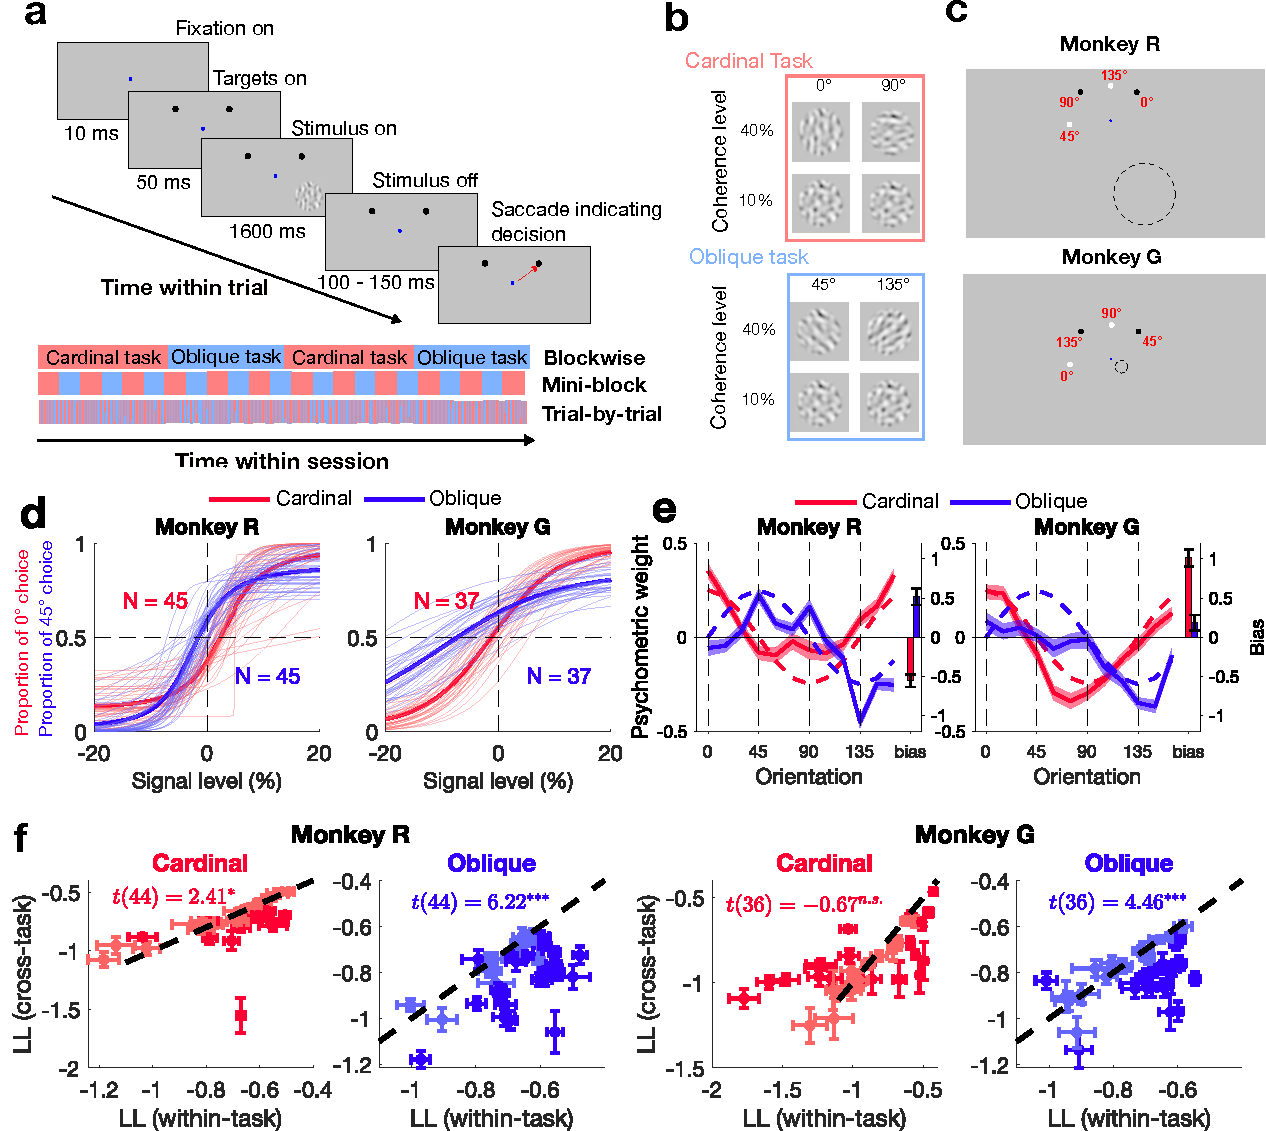
\includegraphics[width=0.8\linewidth]{figures_v2/v2_Figure_2_exp_behav_interleaved.pdf}
    \caption[Experimental design and behavior.]{\textbf{Experimental design and behavior.}
    \textbf{a}: Task design. Saccade targets were shown before the stimulus to cue the animal about task context. After 1.6 seconds of stimulus onset and a random delay, the animals made a saccade to one of the targets to report their decision about orientation. Bottom: Two tasks were interleaved either blockwise or randomly sampled on a trial-by-trial basis.
    \textbf{b}: Examples of visual stimuli.
    \textbf{c}: Layout of saccade targets and stimulus outline (dashed circle represents stimulus location and was not actually shown).
    \textbf{d}: Psychometric curves of all task-switching sessions.
    \textbf{e}: Psychometric orientation kernels. Dashed lines: ideal observer predictions. Solid lines: across-sessions average. Shaded areas: the standard error of the mean across sessions.
   
    \textbf{f}: Cross-predicting choice to evaluate switching of task strategy. x-axis: prediction log-likelihood with orientation kernel inferred from trials of the same task; y-axis: based on orientation kernel inferred from the other task. Each data point represents a single session, and the error bars indicate the standard error of the mean across 20 cross-validation folds. Data points marked with a darker color represent individual sessions with significantly higher within-task prediction performance. 
    }   
    \label{fig:Figure2_behav}
\end{figure}
We trained two rhesus macaque monkeys to perform between two coarse orientation discrimination tasks: the cardinal task was to discriminate between $0^\circ$ and $90^\circ$, while the oblique task was between $ 45^\circ$ and $135^\circ$ (Fig.~\ref{fig:Figure2_behav}b). The neural and behaviroal data was previously reported in \textcolor{red}{LIU et al.}. After the animals learned single tasks, we trained them to switch between two tasks within a single session (Fig.~\ref{fig:Figure2_behav}a). The visual stimuli were dynamic noise whose orientation energy was varied to manipulate signal strength \cite{nienborg2014decision, bondy2018feedback,lange2023weak} (Fig.~\ref{fig:Figure2_behav}b). In each trial, stimulus was shown for 1.6 s (16 different image frames), and then the monkeys reported a choice by making a saccade to one of two targets (Fig.~\ref{fig:Figure2_behav}a). Importantly, the two saccade targets differed in position and luminance between the two tasks (Fig.~\ref{fig:Figure2_behav}c), and the targets were shown before the visual stimulus, to cue the animals about the task context in advance (Fig.~\ref{fig:Figure2_behav}a). In most sessions, the task context was randomized on a trial-by-trial basis, but in a few sessions of monkey G, tasks switched blockwise (block size: 100--200 correct trials), and we used ``mini-blocks" for a subset of sessions of monkey R (block size: 10--50 correct trials) (Fig.~\ref{fig:Figure2_behav}a, bottom). This blockwise design was both to facilitate training and to examine the effect of switching timescale of task switching influenced neural or behavioral signatures.

Both animals could perform both tasks under the task-switching condition (Fig.~\ref{fig:Figure2_behav}d). Decision strategies approximated those of the ideal observer (Fig.~\ref{Figure2_exp_behav}e), but strategies in two epochs (monkey R cardinal, and monkey G oblique) were more consistent with performing a detection task: the decisions were mostly explained by the presence or absence of orientation power at one, not two, task-relevant orientations. Their temporal strategy, as well as our quantification of behavioral performance (\textcolor{red}{LIU et al.}), can be found in Fig.~\ref{fig:Figure_S1_additional_behav}. Overall, monkey G performed the cardinal task significantly better than the oblique task ($t(36) = 20.85$, $p = \num{1.09e-21}$), while monkey R performed both tasks equally well ($t(44) = -1.58$, $p = \num{1.22e-01}$), with imbalanced behavior between tasks in a few sessions (Fig.~\ref{fig:Figure_S1_additional_behav}b). 
 
To assess whether the animals used distinct strategies for the two tasks, we analyzed their orientation kernels, which showed both animals weighed different orientations to make decisions, largely aligning with the ideal orientation kernel for each task (Fig.~\ref{fig:Figure2_behav}f). We further quantified the switching of strategy by predicting choice of held-out trials (20-fold cross-validation) based on orientation kernels inferred from trials of the same task or the other task (Methods). We found in three out of four epochs, within-task prediction performance was significantly higher than cross-task (Paired t-test: monkey R, cardinal, $t(44) = 2.41$, $p = \num{2.00e-02}$; monkey R, oblique, $t(44) = 6.22$, $p = \num{1.61e-07}$; monkey G, cardinal, $t(36) = -0.67$, $p = \num{5.06e-01}$; monkey G, oblique, $t(36) = 4.46$, $p = \num{7.79e-05}$), and many individual sessions show significantly higher within-task prediction (Fig.~\ref{fig:Figure2_behav}f). Together, these behavioral results demonstrate that both monkeys flexibly adjusted their decision strategies depending on task context, consistent with task switching.


\subsection{Information redundancy during task-switching}

We recorded neural activity from V4 while the animals performed task switching between cardinal and oblique tasks. After spike sorting and applying inclusion criteria, each session yielded on average $25.3\pm6.68$ units in monkey R, with $17.49 \pm 6.20$ single units and $7.64 \pm 3.16$ multi-units, and $81.62\pm13.41$ units from each session ($47.03 \pm 10.46$ single units and $34.59 \pm 10.75$ multi-units) for monkey G.  We present results combining single and multi-units in the main text. Analyses based on only single units or multi-units showed consistent agreement (\textcolor{red}{TODO}). We observed little difference in firing rates of units under the two tasks (independent samples t-test, monkey R: $t(2260) = 0.64$, $p = \num{5.23e-01}$; monkey G: $t(6038) = 2.26$, $p = \num{2.37e-02}$; figure~\ref{fig:Figure_S1_basic_neural_histograms}a). Our recorded units were sensitive to both tasks, with 20\% -- 40\% individual units significantly tuned to task-relevant orientations (figure~\ref{fig:Figure_S1_basic_neural_histograms}b). Yielded units were more sensitive (quantified as stimulus $d'$) for the oblique task in monkey R (independent samples t-test, $t(1844) = -2.79$, $p = \num{5.26e-03}$) and more sensitive for the cardinal task in monkey G ($t(5620) = 35.01$, $p = \num{4.71e-243}$). Interestingly, choice-related activity was stronger for the cardinal task in both animals regardless of the training order (monkey R: $t(1946) = 2.87$, $p = \num{4.18e-03}$; monkey G: $t(3254) = 6.63$, $p = \num{3.94e-11}$; Fig.\ref{fig:Figure_S1_basic_neural_histograms}d), presumably reflecting stronger belief signal for the cardinal task.

First, following the same approach as in \textcolor{red}{LIU et al.}, we examined Fisher information redundancy during the interleaved epoch. Across both animals and tasks, we observed positive information redundancy (figure~\ref{fig:Figure_S6_I_redundancy_interleaved_sizeControl_interleaved}, figure~\ref{fig:Figure_S5_I_redundancy_percentage_interleaved_sizeControl_interleaved}). Measured as percentages with respect to the marginal information ($\Is$), the information was $19.47\pm 14.01\%$ (mean $\pm$ s.t.d over sessions)redundant for monkey R, cardinal, and $19.60\pm 11.82\%$ redundant for monkey R, oblique. For monkey G, $\Idelta (\textrm{Percent})$ was $ 29.21\pm  37.28\%$ for the cardinal task, and  $21.89\pm 24.26\%$ for the oblique task. Compared to the late-learning sessions during the learning epoch, the information during the interleaved epoch was less redundant for monkey R ($30.47\pm11.00\%$ for cardinal, $33.61\pm6.58\%$ for oblique), but remained comparable for monkey G  ($22.05\pm27.94 \%$ for cardinal, $ 19.79\pm27.41\%$ for oblique). This suggests that the demand of switching between tasks could have weakly interfered with the belief signal for each individual task. In addition, consistent with late-learning sessions during the learning epoch, we found $\Idelta$ during task performance was significantly higher than that during passive viewing (figure.\ref{fig:Figure_S9_passive_task_Iredundancy_sizeControl}), and increased within a trial in three out of four conditions (figure.~\ref{fig:Figure_S8_withinTrial_Iredundancy_sizeControl}).


We found little relationship between information redundancy and behavioral performance, presumably due to the small dynamic range. No significant relationships were found for monkey G. For monkey R, we found information redundancy was positively associated with performance (figure~\ref{fig:Figure_S6_I_redundancy_interleaved_sizeControl_interleaved}), again explained by even higher $\Is$ rather than decrease of $\Ir$ (figure~\ref{fig:Figure_S7_FisherInfo_sizeControl_nobehav}). However, unlike during the learning epochs, we did not observe significant relationships between $\Idelta (\textrm{Percent})$ and behavior (figure~\ref{fig:Figure_S5_I_redundancy_percentage_interleaved_sizeControl_interleaved}).


In summary, information redundancy of population response during task-switching was comparable to when tasks were performed separately \textcolor{red}{LIU et al}. These results are consistent with predictions of the Bayesian generative framework and indicate that the task-relevant belief signals of both tasks modulate neural responses under the corresponding task context. However, these neural signatures alone can not reflect task-switching, because belief signals that are intermediate between two tasks, which do not switch between task contexts, would also lead to the same outcome for information redundancy. To directly test whether population responses of sensory neurons reconfigure with task context, we next defined two neural signatures of task switching.

\subsection{Higher information redundancy under the same task context during task switching}
\begin{figure}
    \centering
    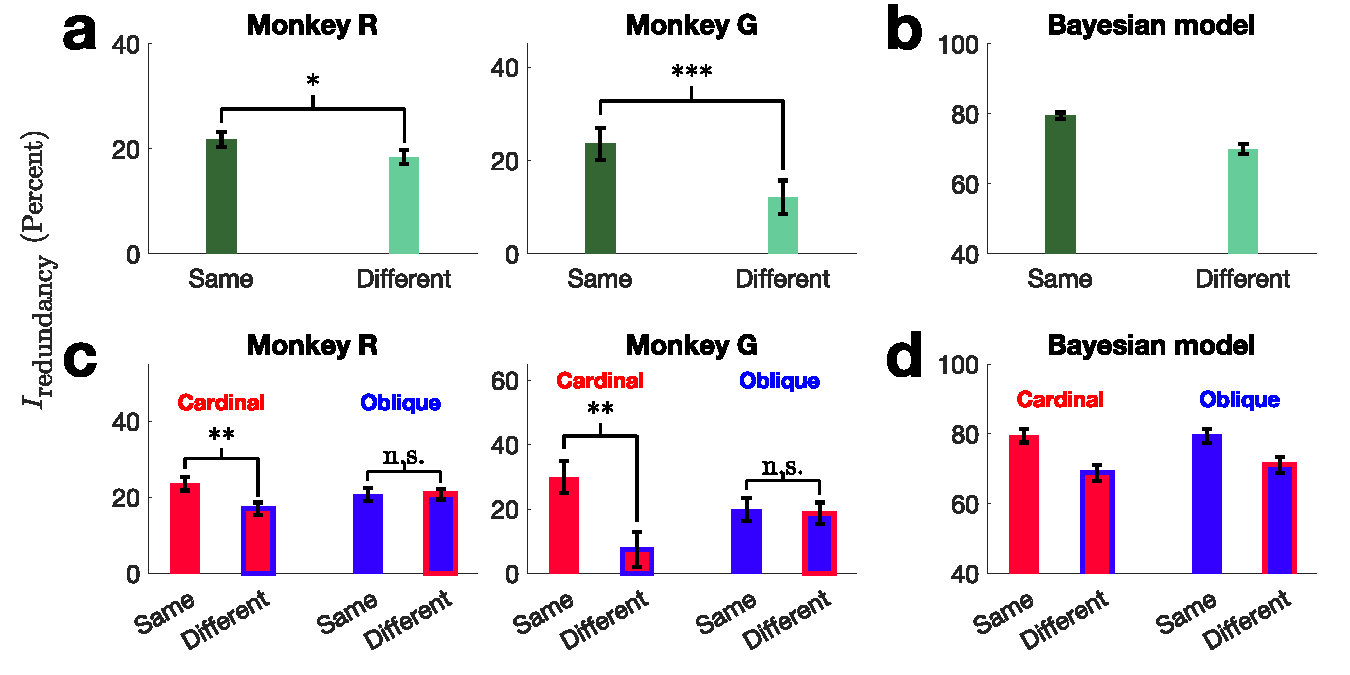
\includegraphics[width=0.8\linewidth]{figures_v2/v2_Figure_3_informationRedundancy_percent.pdf}
    \caption{\textbf{Information redundancy was higher under the same task context.} \textbf{a}: Information information measure as percentage of the shuffled linear Fisher information in both animals. The "same" information redundancy with respect to each task was computed based on the covariance matrix from the same task context, whereas the "different" redundancy was based on covariance matrix from the other task context. Redundancy for cardinal and oblique tasks were averaged to reveal the overall effect. The height of bars indicate average, and the error bars indicate \gls{sem} across sessions. The asterisks indicate significance levels of paired t-test (*: $p < 0.05$; **: $p < 0.01$; ***: $p < 0.001$).
    \textbf{b}: Information information measure as percentage of the shuffled linear Fisher information in the Bayesian model.  \textbf{c} and \textbf{d}: Same as \textbf{a} and \textbf{b}, but presenting two tasks separately.}
    \label{fig:Figure_3_redundancy_percent}
\end{figure}

%%%%% Explain same v.s. different information redundancy 

%%%%% Describe the two-bar results
In both animals, information redundancy under the same task context was significantly higher than information redundancy under the different task context (Fig.~\ref{fig:Figure_3_redundancy_percent}a; monkey R $t(37) = 2.52$, $p = \num{1.60e-02}$; monkey G $t(36) = 3.70$, $p = \num{7.19e-04}$). These results are consistent with predictions of generetive Bayesian model (Fig.~\ref{fig:Figure_3_redundancy_percent}b), and the opposite of the classic framework. Moreover, we did not observe any significant effect of switching timescale, and even sessions with random trial-by-trial task switching showed neural signature of task switching (figure~\ref{fig:Figure_S10_redundancy_percent_bytimescale}), suggesting that the information redistribution process by generative Bayesian inference can be as flexible as adapting to the change of task context within a few seconds. 

%%%%% Describe the four-bar results
Interestingly, unlike in the model where results were symmetric between two tasks (Fig.~\ref{fig:Figure_3_redundancy_percent}d), we observed asymmetry in our empirical data, and such asymmetry was consistent between the two animals (Fig.~\ref{fig:Figure_3_redundancy_percent}c). In both animals, information redundancy with respect to the cardinal task under the cardinal context was significantly higher than that under the oblique context (Fig.~\ref{fig:Figure_3_redundancy_percent}c, red bars; One-sample t-test: monkey R: $t(37) = 3.85$, $p = \num{4.50e-04}$; monkey G:  $t(36) = 3.19$, $p = \num{2.91e-03}$)). However, information redundancy with respect to the oblique task did not show significant differences across task contexts (Fig.~\ref{fig:Figure_3_redundancy_percent}c, blue bars; One-sample t-test: monkey R: $t(37) = 0.26$, $p = \num{7.93e-01}$; monkey G:  $t(36) = 0.11$, $p = \num{9.13e-01}$)).

Information redundancy without normalization by $\Is$ showed consistent results but with more variability across sessions (figure~\ref{fig:Figure_S3_I_redundacy_raw}b). Also, the above analysis combined across coherence levels within each session (\hyperref[sec_ch2:cross_fisher]{Method}), and results from individual coherence levels were consistent (figure~\ref{fig:Figure_S2_empirical_barplot_perCohr}).

%%%%%% I_cross v.s. I real results from the thesis chapter
%In both animals, $\Ir$ was significantly less than $\Icross$ for the cardinal task, with on average $13.58\%$ of difference for monkey R, and $21.27\%$  difference for monkey G (paired t-test: monkey R: $t(37) = -4.14$, $p = \num{1.91e-04}$; monkey G: $t(36) = -3.44$, $p = \num{1.47e-03}$). However, no difference was observed between oblique $\Ir$ and $\Icross$ (monkey R: average difference: $-4.34\%$, $t(37) = 1.60$, $p = \num{1.18e-01}$; monkey G: average difference: $-6.00\%$, $t(36) = 0.20$, $p = \num{8.41e-01}$). 


% \subsection{Neural signature of task-switching in generative Bayesian inference model}
% \begin{figure}[h!]
%     \centering
%     
\includegraphics[width=0.8\linewidth]{figures/Figure_2_simple_simulation.pdf}
%     \caption[Linear Fisher information in a generative Bayesian model simulation of ideal task switching.]{\textbf{Linear Fisher information in a generative Bayesian model simulation of ideal task switching.}
%     \textbf{a}: Diagram of Bayesian model with a prior on task context. The prior layer has two variables: $p(\textrm{cardinal})$ and $p(\textrm{oblique})$, which always sum up to 1. 
%     \textbf{b}: Psychometric curves of the model for cardinal and oblique task before ($\delta = 0$) and after learning ($\delta = 0.08$). 
%     \textbf{c,d}: Formulas and simulation results for comparing effect of covariance from two task contexts on linear Fisher information.
%     \textbf{c}: Formulas to compute $\Icross$ for two tasks. Red variables are computed from responses under the cardinal context, while blue indicates oblique variables.
%     \textbf{d}: Top: $\Ir$ and $\Icross$ for two tasks before and after learning. Bottom: Percentage of limited information with respect to $\Icross$ ($100 * \frac{\Icross - \Ir}{\Icross}\%$).
%     Error bars indicate the 68\% confidence interval across 1000 random samples of synthetic neurons.
%     \textbf{e,f}: Formulas and simulation results for comparing effect of covariance on information redundancy.
%     \textbf{e}: Formulas to compute $\Idelta$ and $\Ideltacross$ for the cardinal task. The formulas for oblique task are symmetric to the cardinal ones.
%     \textbf{f}: Top: $\Idelta$ and $\Ideltacross$ measured as percentage with respect to $\Is$ or $\Ishufflecross$ ($100 * \frac{\Is - \Ir}{\Is}\%$). Bottom: Difference between within and cross percentages.}
%     \label{fig:Figure_2_simple_simulation}
% \end{figure}
% 

% We focused on how task-switching modulates the covariance matrix and its impact on linear Fisher information, the central distinction between the classic and the generative framework. 
%  Specifically, we used trials with orientation signals (coherence level $>$ 0\%) to compute tuning for each task, and the covariance from zero-coherence trials. In those trials, the task context was cued by the location and luminance of the saccade targets(Fig.~\ref{fig:Figure_2_simple_simulation}c), but the stimulus was kept the same across contexts. When we combine the cardinal tuning curve and the covariance from the oblique context, we can define a new measure ``cross'' linear Fisher information for the cardinal task. Similarly, we can compute ``cross'' linear Fisher information for the oblique task by combining the oblique tuning with the covariance from the cardinal context (Fig. \ref{fig:Figure_2_simple_simulation}c). When we compare the ``cross'' linear Fisher information and the real linear Fisher information, the only difference is the context cue in the zero-coherence trials. Therefore, the difference between them reflects the effect of feedback signals about the task context.  If the covariance of neurons reflects beliefs and the beliefs are switching between tasks, as predicted by the generative framework, then $\Icross$ would be higher than $\Ir$. This is because the task-specific belief signal increases variability along the task-relevant tuning axis, thereby introducing stronger information-limiting correlations.



% As in Chapter 2, we randomly sampled a subset of synthetic neurons (32 out of 256), and applied bias-correction for estimates of both $\Ir$ and $\Icross$ (\hyperref[sec_ch2:cross_fisher_bias_correction]{Methods}). Consistent with the prediction of the generative inference framework, $\Ir$ was nearly 40\% less than $\Icross$ in the synthetic data after, but not before, learning (Fig. \ref{fig:Figure_2_simple_simulation}d). Thus, we validated that the relative difference between $\Ir$ and $\Icross$ can reflect the neural signature of task-switching.

% We next asked how task switching should influence information redundancy. Following the same logic as above, we used the correct task tuning and the covariance from the other task context to define ``cross information redundancy'' ($\Ideltacross$), measured as the difference between $\Ishufflecross$ and $\Icross$ (Fig. \ref{fig:Figure_2_simple_simulation}e, \hyperref[sec_ch2:cross_fisher]{Methods}), and focused on the relative redundancy as a percentage of $\Ishufflecross$ ($\Ideltacross (\textrm{Percent})$). Similarly, we computed $\Ideltawithin (\textrm{Percent})$, and used the difference between within and cross information redundancy as another neural signature of task switching. The difference between $\Icross$ and $\Ir$ was contributed by both covariance and variance, but the relative redundancy is normalized by the shuffled information, thus removing the contribution from variance.
% Before learning, 60\% of the information in synthetic neurons was redundant due to image computation inequality (Fig. \ref{fig:Figure_2_simple_simulation}f, left), but no difference was observed between information redundancy introduced by the covariance from the true task ($\Ideltawithin (\textrm{percent})$) and that introduced by covariance from the other task ($\Ideltacross (\textrm{percent})$) (Fig. \ref{fig:Figure_2_simple_simulation}f, left). However, after learning, within-task information redundancy increased to 80\% and exceeded cross-task redundancy by about 10\% (Fig. \ref{fig:Figure_2_simple_simulation}f, right).


% In summary, our Bayesian generative model predicts covariance changes with task context. Notably, covariance was estimated with only zero-coherence trials. Thus, the feedforward pathway was kept consistent, and any difference in the covariance was due to feedback signals. This implies the feedback signals in the current task context in the Bayesian model limit, rather than enhance, the information for the current task, and introduce more information redundancy, compared with feedback signals in a different task context. Next, we aimed to test whether these two neural signatures (one on linear Fisher information, one on information redundancy) of switching existed in our empirical data.
% \subsection{Empirical data shows supporting evidence, but asymmetry between tasks}
% \begin{figure}
%     \centering
%     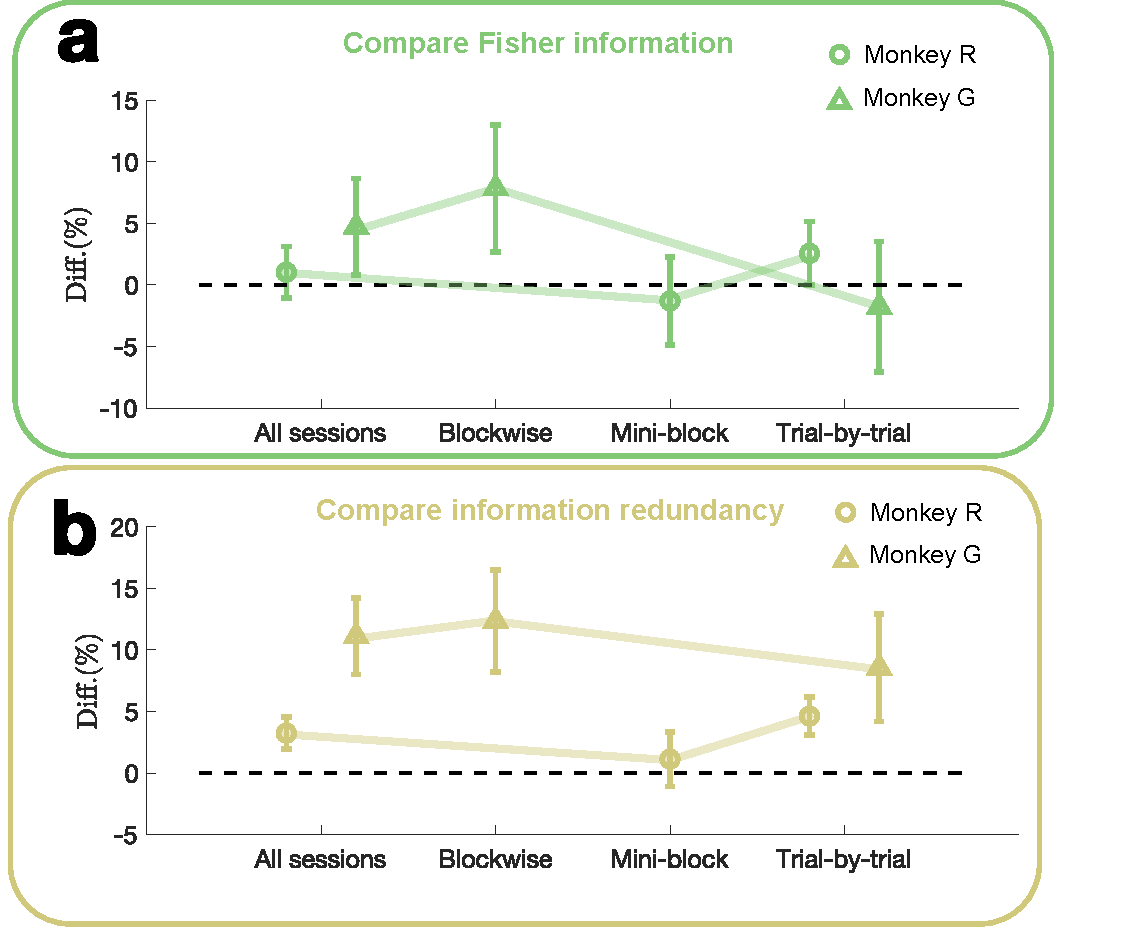
\includegraphics[width=0.8\linewidth]{figures/Figure_9_empirical_avg_block_trial.pdf}
%     \caption[Neural signature of switching averaged across two tasks, as a function of switching timescale.]{ \textbf{Neural signature of switching averaged across two tasks, as a function of switching timescale.}\textbf{a}: The relative difference between $\Icross$ and $\Ir$. Symbols and error bars indicate the mean and \gls{sem} across all sessions, blockwise sessions, and trial-by-trial sessions. Circle symbols indicate results for monkey R and triangle symbols indicate results for monkey G. \textbf{b}: Similar to \textbf{a}, but presenting the difference between $\Ideltawithin$ (Percent) and $\Ideltacross$ (Percent). }
%     \label{fig:Figure_9_empirical_avg_block_trial}
% \end{figure}

% \begin{figure}
%     \centering
%     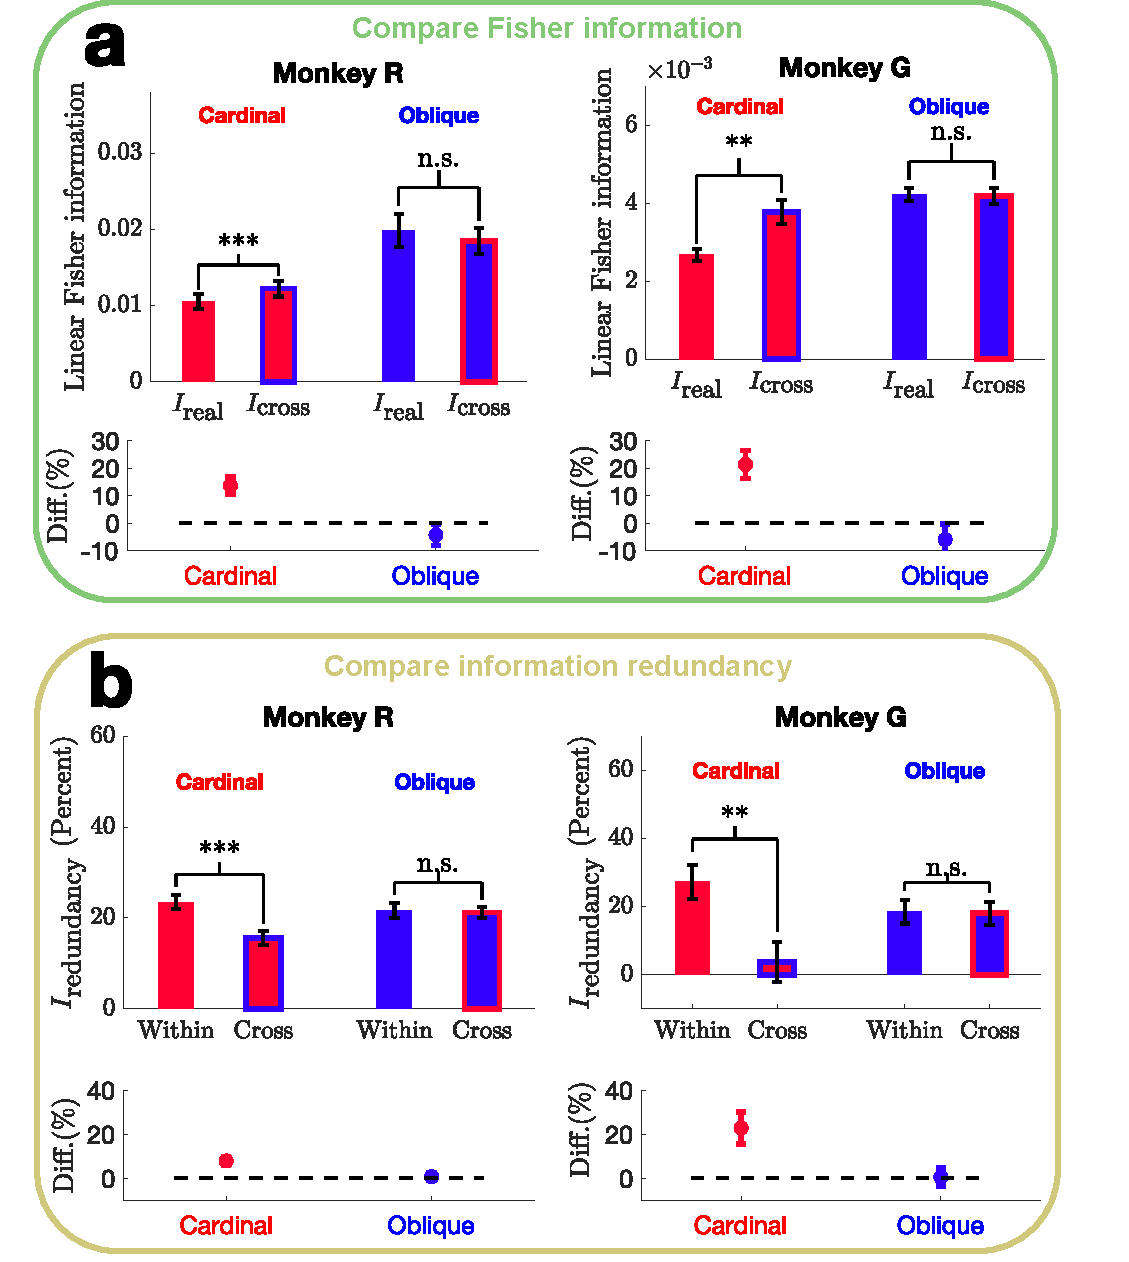
\includegraphics[width=0.8\linewidth]{figures/Figure_3_empirical_barplot.pdf}
%     \caption[Linear Fisher information under task switching in the empirical data.]{\textbf{Linear Fisher information under task switching in the empirical data.}\textbf{a}: Compare $\Ir$ and $\Icross$ for two animals. Top: average and \gls{sem} of Fisher information across sessions. Bottom: difference between $\Icross$ and $\Ir$ as the percentage of $\Icross$. \textbf{b}: Compare information redundancy (as the percentage of $\Is$) introduced by the within-task covariance matrix and the cross-task covariance matrix. Top: average and \gls{sem} of $\Ideltawithin$ and $\Ideltacross$ across sessions. Bottom: difference between $\Ideltawithin$ and $\Ideltacross$. In this figure, each bar represents the mean across sessions. For each session, the metric was computed as a weighted average across coherence levels, and these session-level values were then averaged. (\hyperref[sec_ch2:cross_fisher]{Method}). Results with separated coherence levels show consistent patterns (figure~\ref{fig:Figure_S2_empirical_barplot_perCohr}). }
%     \label{fig:Figure_3_empirical_barplot}
% \end{figure}



% We next computed Fisher information metrics to test the neural signatures of task switching predicted by the Bayesian model (Fig.~\ref{fig:Figure_9_empirical_avg_block_trial}, all sessions). The timescale of task-switching had inconsistent effects on the neural data. For monkey G, it appeared that sessions of block-wise switching mostly accounted for the effects of the information-based neural signature (Fig.~\ref{fig:Figure_9_empirical_avg_block_trial}a, triangle symbols), and the redundancy-based neural signature showed a similar, but weaker trend (Fig.~\ref{fig:Figure_9_empirical_avg_block_trial}b, triangle symbols). It was the opposite for monkey R: trial-by-trial switching introduced slightly stronger neural signatures.




% We also found that when only zero-coherence trials were used to assess redundancy, it was comparably redundant (monkey R, cardinal $Mean = 23.43\%$; monkey R, oblique: $Mean = 21.70\%$; monkey G, cardinal: $Mean = 27.25\%$; monkey G, oblique: $18.55\%$) to those computed with non-zero coherence trials, suggesting redundancy was primarily driven by belief signals, which were as strong when evidence was ambiguous. 



% In summary, our empirical results demonstrated neural signatures of task-switching: the covariance structure of population responses can flexibly switch within-session (and even trial-by-trial) in a way that limits information and introduces \emph{more} information redundancy for the currently performed task at the moment. These signatures align with predictions of the Bayesian generative model. However, the effects were evident only for the cardinal task. This asymmetry echoes the behavioral cardinal bias observed in our animals (Fig.~\ref{fig:Figure1_behav}) and motivated further investigation into the underlying sources of task-dependent asymmetry described in the following sections.

\subsection{Bayesian inference with more realistic assumptions could replicate asymmetry between tasks}
\begin{figure}[h!]
    \centering
    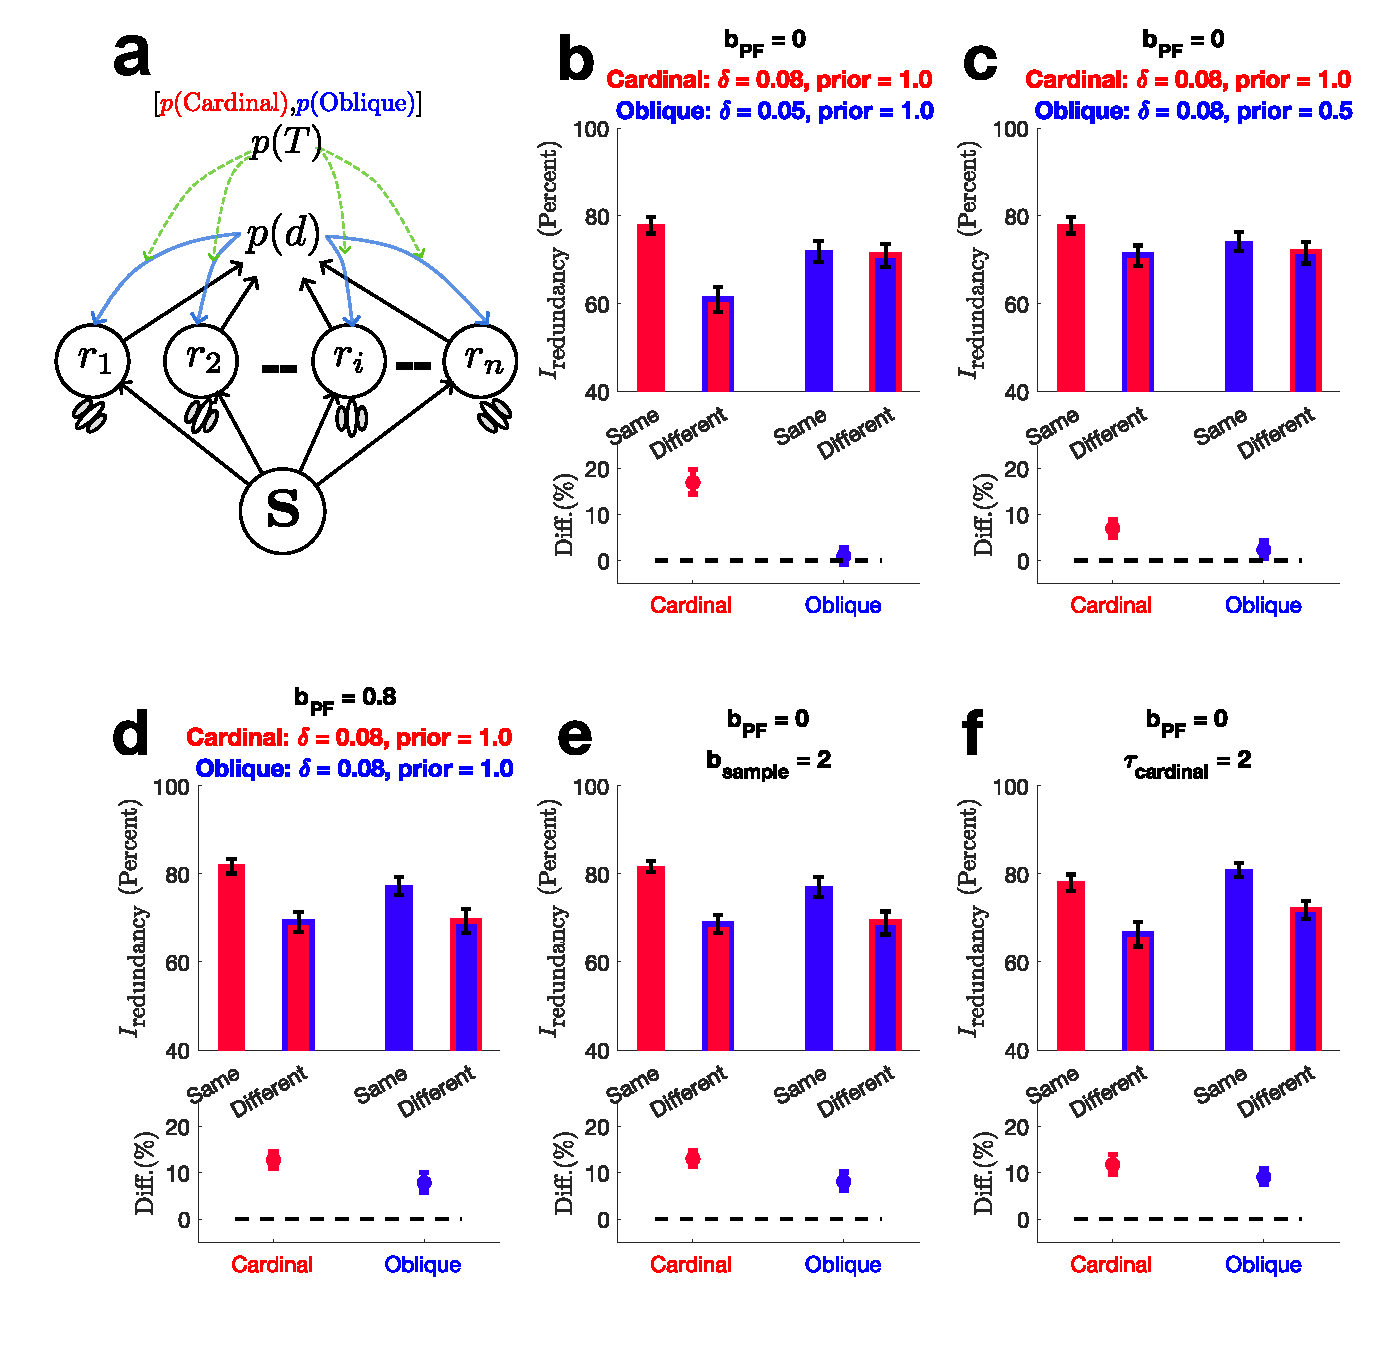
\includegraphics[width=0.8\linewidth]{figures_v2/v2_Figure_4_informationRedundancy_simulation_nonIdeal.pdf}
    \caption[Model simulation of imperfect task-switching.]{\textbf{Model simulation of imperfect task-switching.}  \textbf{a}: Diagram of Bayesian model with a prior on task context. The prior layer has two variables: $p(\textrm{cardinal})$ and $p(\textrm{oblique})$, which always sum up to 1. 
    In each panel from \textbf{b} to \textbf{c}, the top shows information redundancy (percent) under the same or different task context for each task, and their differences was shown at the bottom for better illustration. \textbf{b}: Simulation of stronger learning strength for the cardinal task than the oblique. \textbf{c}: Simulation of imperfect switching of task strategy. \textbf{d}: Simulation of neuron population that over-represents cardinal orientations. \textbf{e}: Simulation of sub-sampling a uniform population such that more synthetic neurons prefer the cardinal orientations. \textbf{f}: Simulation of sub-sampling a uniform population such that cardinal and oblique sensitivity are balanced,  but more neurons whose orientation preference is closer to $0^\circ$ for the cardinal task.}
    \label{fig:Figure_4_nonideal_simulation}
\end{figure}

We used the same hierarchical Bayesian inference model described in \citet{haefner2016perceptual} and \textcolor{red}{LIU et al.} and extended it to perform task switching between cardinal and oblique discrimination tasks. On top of the decision variable, the model incorporates a higher-level layer of variable that represents prior beliefs about the task context (Fig. \ref{fig:Figure_4_nonideal_simulation}a, \hyperref[sec_ch2:ideal_simulation]{Methods}). 

While our initial modeling results showed symmetric neural signatures of switching between the two tasks, we found that the neural signatures of task-switching for the monkeys were not symmetric. So what could explain the discrepancy between the model simulation and our empirical results, as well as the asymmetry between cardinal and oblique tasks? A likely reason is that our original simulation was over-simplified, and therefore did not capture several complexities of real neural systems.

In the previous simulation, our Bayesian model employed ideal task strategies. The model learned two tasks equally well and switched between them perfectly. Also, the orientation preference of the synthetic neurons uniformly tiles the orientation space. However, we reasoned that the reality deviated from these assumptions.
The strategy of animals deviates from the ideal ones (Fig.~\ref{fig:Figure2_behav}e), and the switching between two tasks is very likely to be imperfect (Fig.~\ref{fig:Figure2_behav}f). Additionally, the performance of the two tasks was often unequal, with better cardinal performance in most sessions (Fig.~\ref{fig:Figure_S1_additional_behav}b), consistent with the cardinal bias phenomenon observed in humans and non-human primates~\citep{appelle1972perception, nasr2012cardinal}. Moreover, there has been some evidence for orientation anisotropy in macaque visual cortices, with more neurons preferring cardinal orientations~\citep{mansfield1974neural, nasr2012cardinal, fang2022orientation}. The sampling of neurons by Utah arrays is also effectively random and likely non-uniform, introducing further biases into the recorded populations.

Taken together, these considerations suggest that the mismatch between model and data is not a failure of the generative framework, but a reflection of unmodeled biological constraints and behavioral asymmetries. In the following section, we extend our Bayesian model with simple but biologically motivated modifications that incorporate these factors. We then test whether these modifications can reproduce the asymmetric patterns observed in the empirical data.


\subsubsection{Learning strength} From \textcolor{red}{Liu et al}, we have shown information redundancy in our Bayesian model is contributed by task learning. Therefore, we first examined the effect of unequal learning between the two tasks. In the model, learning strength was controlled by a parameter $\delta$ that determines the strength of interdependence between sensory neurons and the decision variable (\hyperref[sec_ch1:Hierarchical Bayesian inference model]{Chapter 2, Methods}, also see~\citet{haefner2016perceptual} for details). To mimic the behavioral asymmetry observed in our animals, we assigned a higher $\delta$ for the cardinal task ($\delta_\textrm{cardinal} = 0.08$) than the oblique ($\delta_\textrm{oblique} = 0.05$), while keeping all of the other parameters identical to those in the ideal simulation.
This modified simulation showed strong asymmetry in information redundancy across two tasks, consistent with the empirical data: for the cardinal task, large differences between between $\Ideltacross$ and $\Ideltawithin$ (Fig.~\ref{fig:Figure_4_nonideal_simulation}b, red bars). In contrast, for the oblique task, these differences were negligible and indistinguishable from zero (Fig.~\ref{fig:Figure_4_nonideal_simulation}b, blue bars). Thus, introducing asymmetric learning strength into the Bayesian model was sufficient to capture the key features of empirical results.

\subsubsection{Task prior}
In all the above simulations, we assumed complete knowledge about the correct task context, reflected in the task prior parameter being 1 for the correct task. Next, we examined the effect of the prior over the task-context on information redundancy, which shapes the profile of the interdependence between sensory and decision layers, i.e., task-solving strategy and the structure of feedback signals. In this simulation, we keep other parameters equal across tasks and set the priors to be $[p_\textrm{cardinal} = 1, p_\textrm{oblique} = 0]$ for the cardinal task, and $[p_\textrm{cardinal} = 0.5, p_\textrm{oblique} = 0.5]$ for the oblique task (\hyperref[sec_ch2:nonideal_simulation_test]{Methods}). Under these conditions, the model is biased towards cardinal context, employs an ideal strategy to perform the cardinal task, while employing a mixed strategy (i.e., an intermediate strategy between cardinal and oblique) for the oblique task. As a result, switching from cardinal to oblique context was inherently imperfect.

This manipulation also reproduced the asymmetry observed in our empirical data: both neural signatures based on linear Fisher information and information redundancy showed strong effects for the cardinal task but minimal effects for the oblique (Fig.~\ref{fig:Figure_4_nonideal_simulation_test}c). However, compared with the simulation with unequal learning (Fig.~\ref{fig:Figure_4_nonideal_simulation_test}b), the asymmetry introduced by imperfect task prior was slightly weaker..


\subsubsection{Biased population}  Lastly, we test whether an imbalanced population of units could account for the observed asymmetry. In this simulation, a different population of sensory neurons was generated such that more synthetic neurons prefer cardinal orientations (\hyperref[sec_ch2:nonideal_simulation_test]{Methods}), while the models performed two tasks with equal learning strength and prior. This manipulation produced only modest difference in the model's performance and asymmetry between the two tasks (Fig.~\ref{fig:Figure_4_nonideal_simulation}d). The asymmetry was much weaker compared to the other two simulations above. Also, in contrast to the empirical data, the oblique task shows a strong difference between $\Ideltacross$ and $\Ideltawithin$. Thus, while orientation anisotropy can introduce bias towards the cardinal task, this factor alone cannot fully explain the empirical asymmetry we observed.

% \begin{figure}
%     \centering
%     
\includegraphics[width=0.8\linewidth]{figures/Figure_5_sampleneuron_simulations.pdf}
%     \caption[Simulation of sub-sampling neurons from an existing population.]{\textbf{Simulation of sub-sampling neurons from an existing population.}In each panel, the top shows the difference between $\Icross$ and $\Ir$ as a percentage of $\Icross$, and the bottom shows the difference between $\Ideltawithin \textrm{(Percent)}$ and $\Ideltacross \textrm{(Percent)}$. \textbf{a}: Results from the original population for comparison. \textbf{b}: Results from sub-sampling the population such that more synthetic neurons prefer the cardinal orientations. \textbf{c}: Results from a sub-sampled population with balanced cardinal and oblique sensitivity, but more neurons whose orientation preference is closer to $0^\circ$ for the cardinal task.}
%     \label{fig:Figure_5_sampleneuron_simulation}
% \end{figure}

\subsubsection{Non-uniform sampling of units}
Other than the intrinsic cardinal bias of orientation preference of the visual cortex, the random sampling of neurons by Utah arrays could further introduce non-uniformity in orientation preferences. Indeed, we observed an imbalance in terms of orientation preference in empirical data across and within tasks: Units from monkey R were slightly more sensitive to the cardinal task and those from monkey G were more sensitive to the oblique task(figure~\ref{fig:Figure_S1_basic_neural_histograms}b). Furthermore, recorded units from both animals disproportionately preferred $0^\circ$ and $45^\circ$ relative to $90^\circ$ and $135^\circ$ (figure~\ref{fig:Figure_S1_basic_neural_histograms}c). 

To test whether such biased sub-sampling of neurons from an existing population would account for the observed asymmetry in neural signatures, we simulated drawing neurons from a population with uniform orientation preference (\hyperref[sec_ch2:simulate_subsampling]{Methods}). 

Sub-sampling more cardinal-sensitive neurons leads to an asymmetry in terms of the difference between same- and different-task information redundancy (Fig.~\ref{fig:Figure_4_nonideal_simulation}e), and the asymmetry is comparable to the asymmetry introduced by intrinsic bias of the population (Fig.~\ref{fig:Figure_4_nonideal_simulation}d).  On the other hand, only sampling more neurons whose orientation preference is closer to one relevant orientation of the cardinal task, while keeping sensitivities for two tasks balanced, did not introduce any notable effect on information redundancy (Fig.~\ref{fig:Figure_4_nonideal_simulation}f).

Taken together, these results suggest that sampling imbalances towards one task, but not towards a single orientation within a task, can introduce modest asymmetry in neural signatures of task-switching. 

\subsection{Quantitative matching between empirical data and Bayesian model}
\begin{figure}
    \centering
    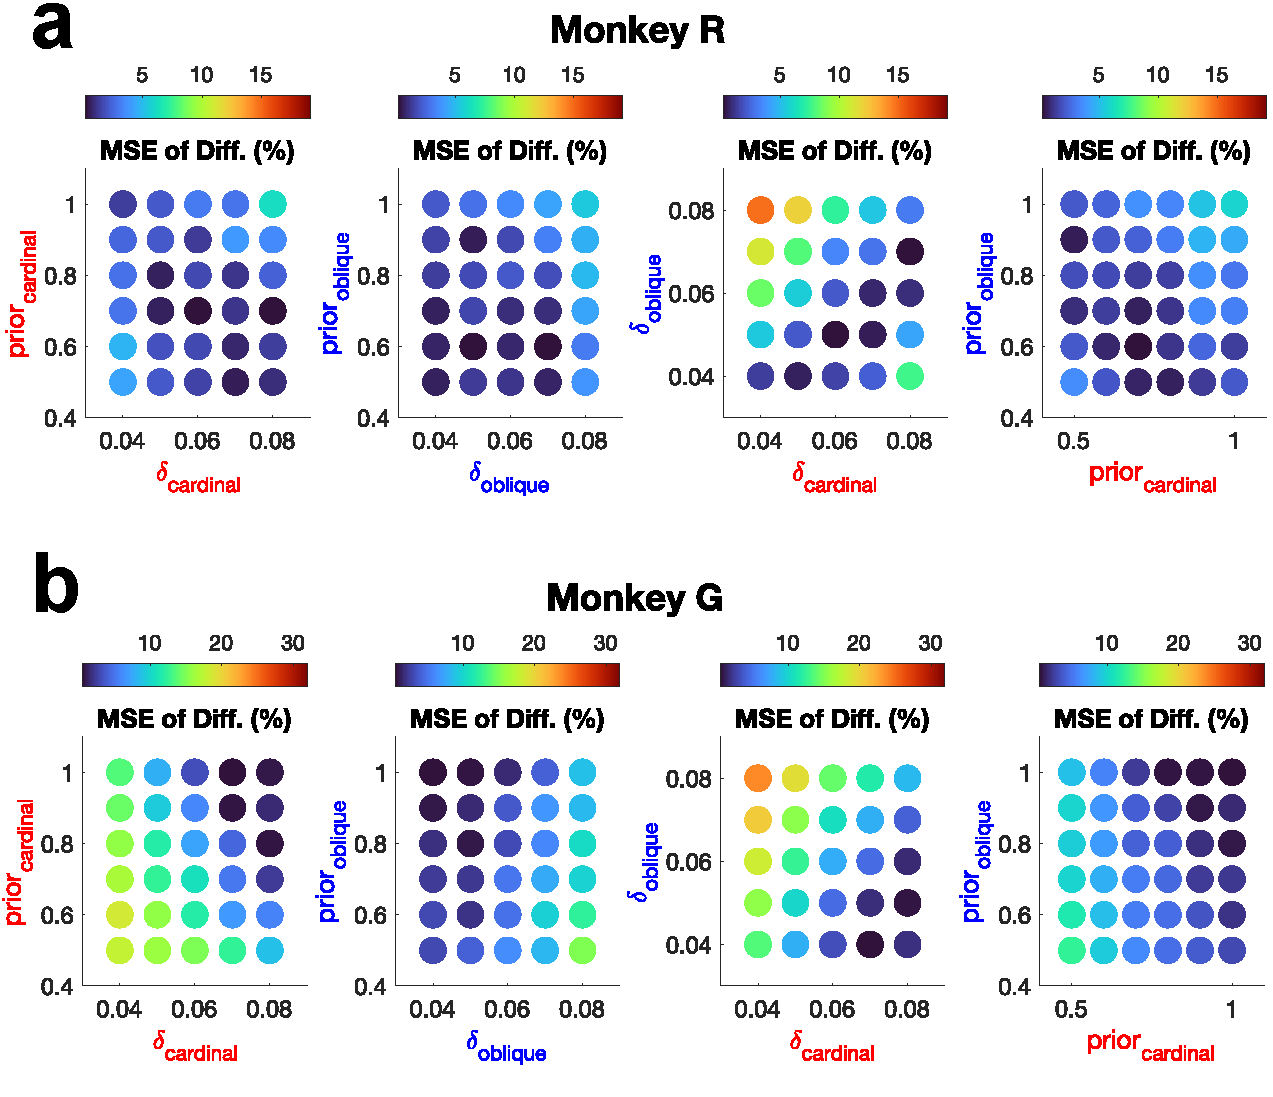
\includegraphics[width=0.8\linewidth]{figures_v2/v2_Figure_5_scatter_largescale_match.pdf}
    \caption{\textbf{Scatter plot of match between simulation and empirical data in four-dimensional parameter space.} For each combination of four parameters ($\delta_{\textrm{cardinal}}$, $\delta_{\textrm{oblique}}$, 
$\textrm{prior}_{\textrm{cardinal}}$ and $\textrm{prior}_{\textrm{oblique}}$),  \textbf{a}: Mean squared error between empirical measurement from monkey R. \textbf{b}: Mean squared error between empirical measurement from monkey G.}
    \label{fig:Figure_5_scatter_match}
\end{figure}
% \begin{figure}
%     \centering
%     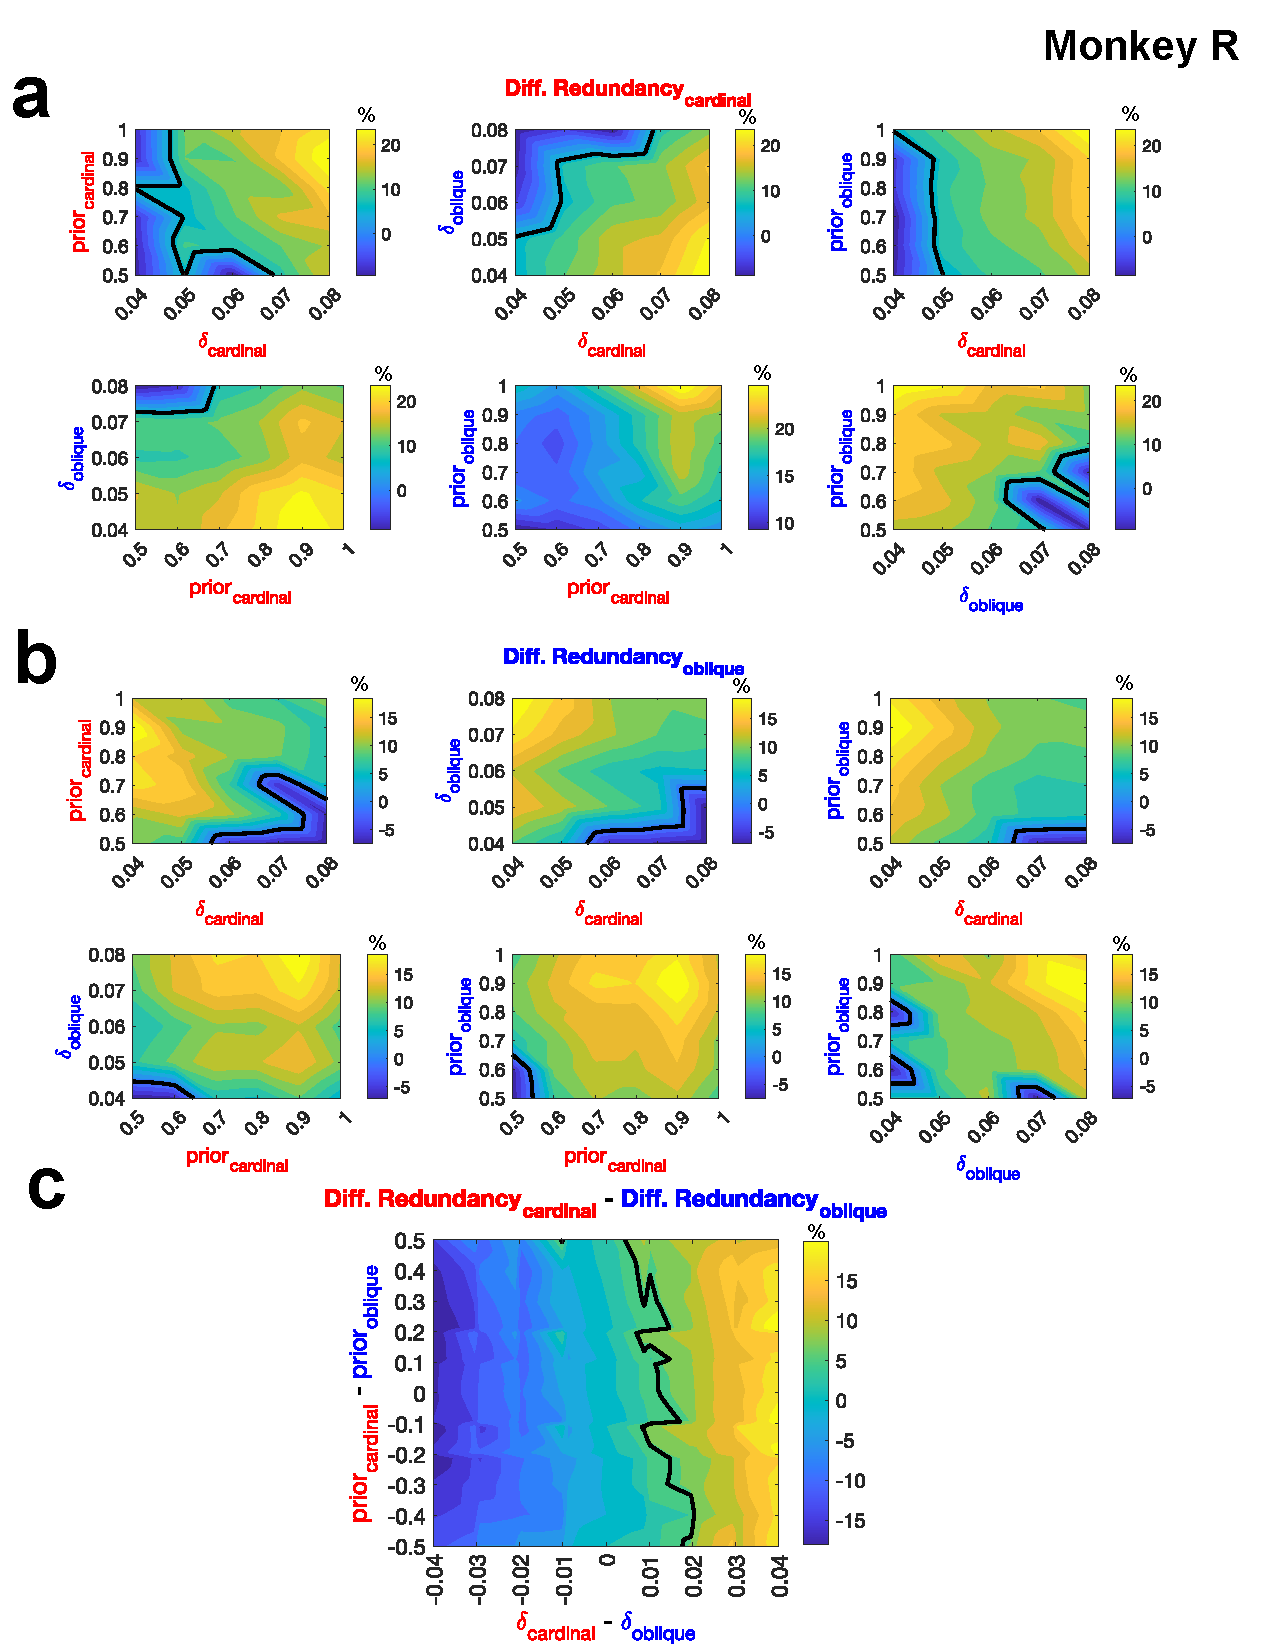
\includegraphics[width=0.8\linewidth]{figures/Figure_6_simulation_4D_redundancy_monkeyR_matched.pdf}
%     \caption[Large-scale simulation of effects of learning strength and task prior parameters on information redundancy for monkey R.]{\textbf{Large-scale simulation of effects of learning strength and task prior parameters on information redundancy for monkey R.} \textbf{a}: Effects of combinations of parameters on the difference between within and cross information redundancy for the cardinal task. Each sub-panel shows a two-dimensional parameter subspace. The black contour indicates the empirical observation for monkey R, averages across sessions. \textbf{b}: Same as \textbf{a} but for the difference in information redundancy for the oblique task. \textbf{c}: Effect of asymmetry of the two parameters between two tasks on the asymmetry of information redundancy. The black contour indicates the empirical asymmetry. All of the heatmaps were smoothed with linear interpolation. }
%     \label{fig:Figure_6_simulation_4D_redundancy_monkeyR}
% \end{figure}

% \begin{figure}
%     \centering
%     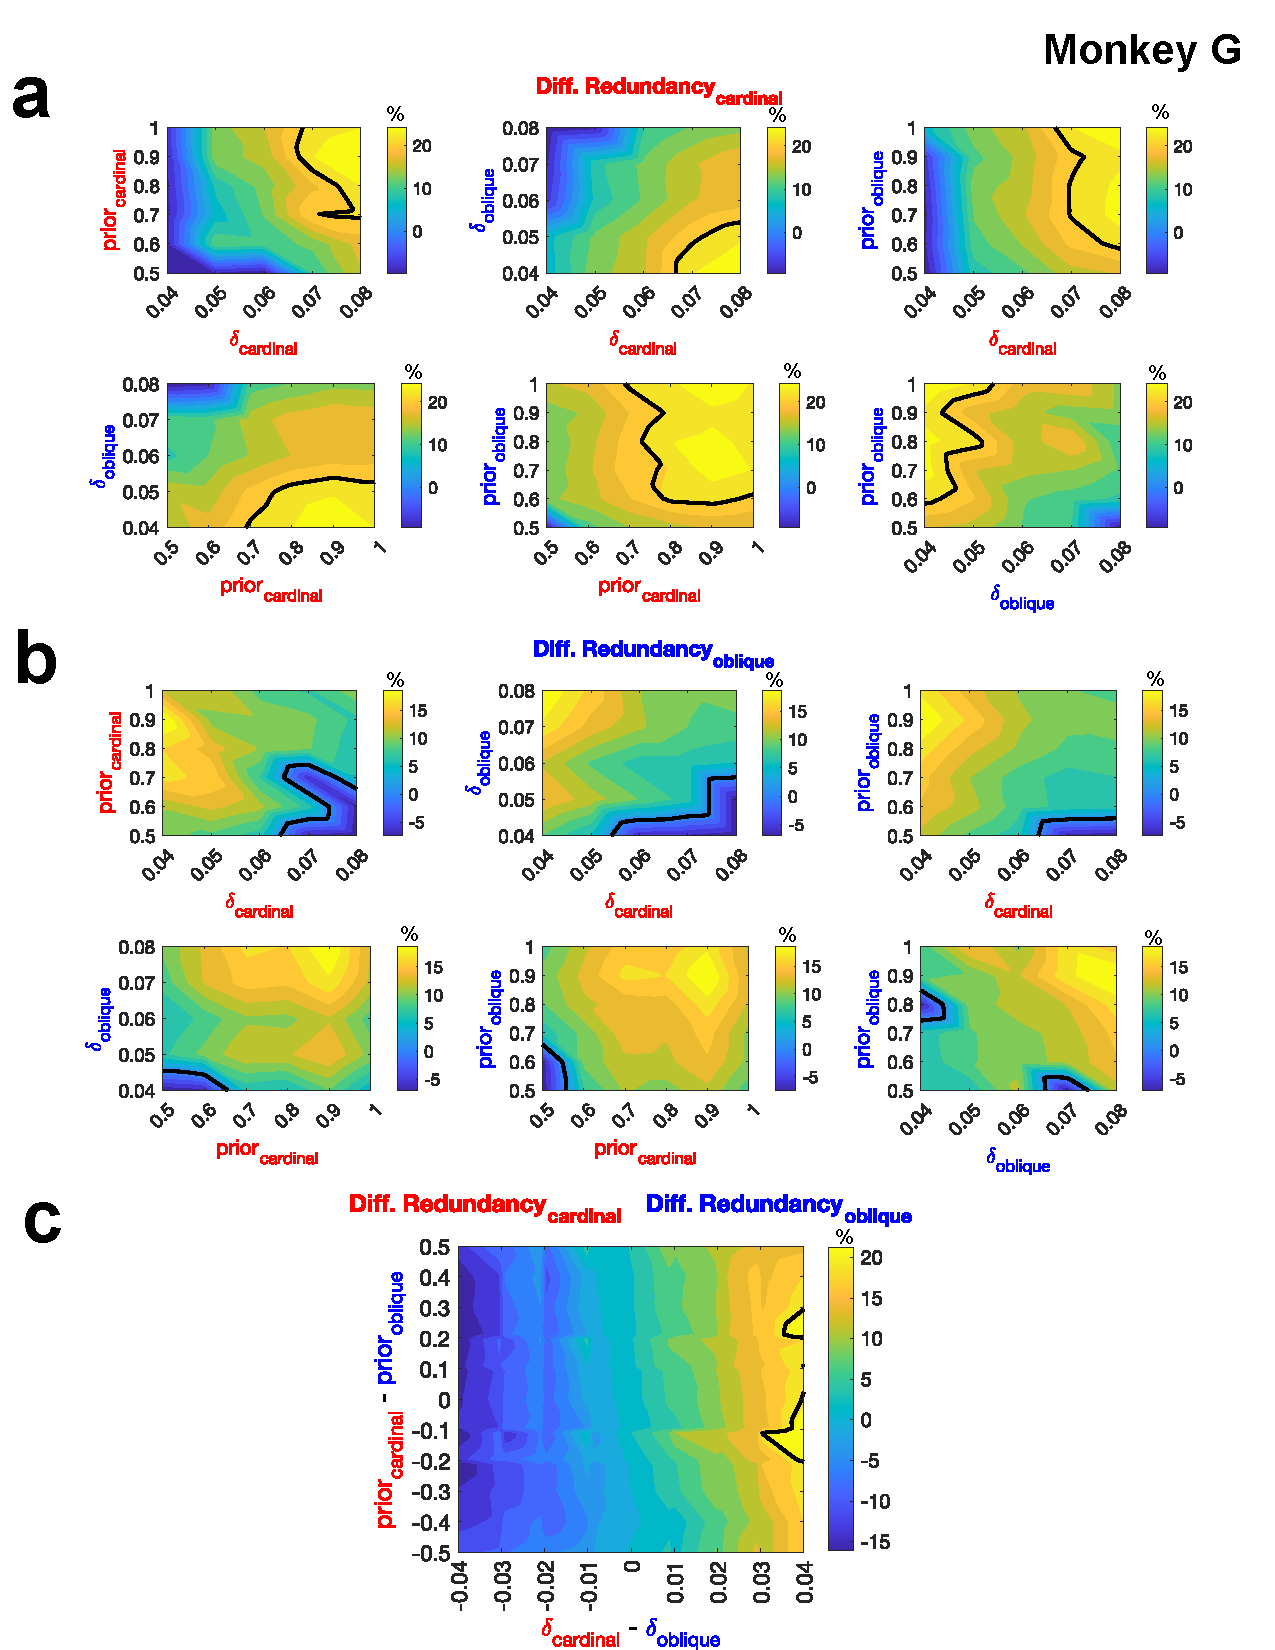
\includegraphics[width=0.8\linewidth]{figures/Figure_6_simulation_4D_redundancy_monkeyG_matched.pdf}
%     \caption[Large-scale simulation of effects of learning strength and task prior parameters on information redundancy for monkey G.]{\textbf{Large-scale simulation of effects of learning strength and task prior parameters on information redundancy for monkey G.}\textbf{a}: Effects of combinations of parameters on the difference between within and cross information redundancy for the cardinal task. Each sub-panel shows a two-dimensional parameter subspace. The black contour indicates the empirical observation for monkey G, averages across sessions. \textbf{b}: Same as \textbf{a} but for the difference in information redundancy for the oblique task. \textbf{c}: Effect of asymmetry of the two parameters between two tasks on the asymmetry of information redundancy. The black contour indicates the empirical asymmetry. All of the heatmaps were smoothed with linear interpolation. }
%     \label{fig:Figure_6_simulation_4D_redundancy_monkeyG}
% \end{figure}

In the preceding section, we demonstrated that several individual manipulations, designed to mimic realistic situations in empirical experiments, such as unequal learning strength, biased task priors, or imbalanced orientation sampling, could qualitatively reproduce key features of our empirical findings. In reality, however, all of these factors could deviate from the most idealized scenario and act simultaneously. To capture this complexity, we next aimed to find the combination of these parameters that best explained the Fisher information results for each animal. To do so, we ran simulations with combinations of four parameters: $\delta_\textrm{cardinal}$, $\delta_\textrm{oblique}$, $\textrm{prior}_\textrm{cardinal}$, and $\textrm{prior}_\textrm{oblique}$ with a population of neurons with realistic cardinal bias ($b_{PF} = 0.8$), subsampled neurons to match tuning statistics for each animal, and then computed the two neural signatures of switching
(\hyperref[sec_ch2:nonideal_simulation_largescale]{Methods}). 

In these large-scale simulations, we found that the two neural signatures of switching, within- and cross-task difference in terms of linear Fisher information, and the difference in terms of information redundancy, were highly correlated with each other ($r(898) =  0.975$ for the cardinal task, and $r(898) =  0.977$ for the oblique). We therefore focused on the neural signature of switching in terms of information redundancy in the following discussions. Heat maps of redundancy differences for each animal are shown in Fig.~\ref{fig:Figure_6_simulation_4D_redundancy_monkeyR} and Fig.~\ref{fig:Figure_6_simulation_4D_redundancy_monkeyG}.

The relationship between information redundancy and the four parameters was broadly consistent across two animals. The difference between $\Ideltawithin$ and $\Ideltacross$ is positively correlated with the learning strength ($\delta$) of the corresponding task, and negatively correlated with the other task. Task priors for both contexts enhance the difference in redundancy, suggesting that as long as the model applies distinct strategies for different tasks, neural signatures of switching should emerge. Notably, when examining the asymmetry in the neural signature as a function of the asymmetry in the parameters, the asymmetry in learning strength exerted a far stronger influence than the asymmetry in prior.

We further demonstrated that the empirical measurements of the redundancy-based neural signature of switching could be quantitatively reproduced by the simulations (see black contours in Fig.~\ref{fig:Figure_6_simulation_4D_redundancy_monkeyR} and Fig.~\ref{fig:Figure_6_simulation_4D_redundancy_monkeyG}). For each animal, we successfully identified parameter combinations (table~\ref{tbl:best_simulation_params}) that best matched the empirical observations (table~\ref{tbl:simulation_match}).

Consistent with the behavioral results that monkey G performed much better for the cardinal task and his oblique orientation had a greater deviation from the ideal, the parameters that best explained monkey G exhibited a pronounced cardinal bias in both $\delta$ and task prior. In contrast, the parameters for monkey R were more balanced across tasks. Consistently, to account for the asymmetry in the neural signature of switching, the imbalance between $\delta_\textrm{cardinal}$ and $\delta_\textrm{oblique}$ had to be substantially larger for monkey G than for monkey R (Fig.~\ref{fig:Figure_6_simulation_4D_redundancy_monkeyR}c and Fig.~\ref{fig:Figure_6_simulation_4D_redundancy_monkeyG}c).



\begin{table}[h!]
    \centering
    \small
    \caption[The empirical and the matched neural signature of switching.]{\textbf{The empirical and the matched neural signature of switching.} Each entry indicates the difference between $\Ideltawithin$ (Percent) and $\Ideltacross$ (Percent).}
    \begin{tabular}{lcccc}
    \toprule
    & Cardinal, empirical & Cardinal, matched & Oblique, empirical & Oblique, matched \\
    \midrule
    monkey R & \makecell{6.67\%} & \makecell{6.71\%} & \makecell{-0.07\%} & \makecell{-0.16\%} \\
    \midrule
    monkey G & \makecell{21.72\%} & \makecell{21.28\%} & \makecell{1.28\%} & \makecell{0.75\%} \\
    \bottomrule
    \end{tabular}
    \label{tbl:simulation_match}
\end{table}

\begin{table}[h!]
    \centering
    \caption[The best combination of parameters to explain empirical observation of each animal.]{\textbf{The best combination of parameters to explain empirical observation of each animal.}}
    \begin{tabular}{lccccc}
        \toprule
        & $\delta_\textrm{cardinal}$ & 
        $\textrm{prior}_\textrm{cardinal}$ &
        $\delta_\textrm{oblique}$ & 
        $\textrm{prior}_\textrm{oblique}$
         \\
         \midrule
         monkey R & 0.06 & 0.60 & 0.04 & 0.80
         \\ 
         \midrule
         monkey G & 0.08 & 1.00 & 0.04 & 0.60 \\
         \bottomrule
    \end{tabular}
    \label{tbl:best_simulation_params}
\end{table}








\section{Methods}\label{sec11}

\subsection{Experimental procedures}
A significant amount of data from this experiment has been reported in \hyperref[sec_ch1:chapter_2]{Chapter 2}, in which detailed experimental procedures can be found (\hyperref[sec_ch1:Experiment procedures]{Chapter 2, Methods}). Here, we briefly summarize the procedures.
\subsubsection{Ethical oversight} 
Experimental procedures were approved by the University Committee on Animal Resources of the University of Rochester and were performed in accordance with the United States National Research Council’s \emph{Guide for the Care and Use of Laboratory Animals} \citep{guide}.
\subsubsection{Subjects}
We used two male adult rhesus macaques (\emph{Macaca mulatta}) for this study. We used 96-channel Utah arrays to record from V4 in the left hemispheres of the subjects.
\subsubsection{Microelectrode array recording and spike sorting}
Signals from Utah arrays were preprocessed by a Grapevine system (Ripple). We then used a customized software \citep{spikesorting_url} to perform spike-sorting. The initial spike sorting procedure yielded $27.16\pm6.58$ units on average for each session of monkey R ($19.13 \pm 6.28$ single units and $8.02 \pm3.17$ multiunits), and on average $92.70 \pm 12.99$ units for monkey G ($53.38 \pm 10.50$ single units and $39.32 \pm 11.76$ multiunits). Single units and multiunits were divided based on the signal-to-noise ratio of spike waveforms.

\subsubsection{RF mapping}
Receptive fields of recorded V4 units were mapped by presenting small sinusoidal gratings (radius = $1.6^\circ$ of visual angle) at a matrix of positions. We then used stimuli that roughly covered the aggregated RF area. The centers and radius of the stimuli were: $center_x = 6.4^\circ$, $center_y = -14.2^\circ$, $radius =  6.4^\circ$ (monkey R); $center_x = 2.1^\circ$, $center_y = -0.3^\circ$, $radius = 1.3^\circ$ (monkey G), in which a positive sign means rightward/upward with respect to the fixation center.

\subsubsection{Visual stimuli} 
The visual stimuli were dynamic white noise images filtered with a spatial frequency band and an orientation band~\citep{nienborg2014decision, bondy2018feedback, lange2023weak}. Stimuli were presented on a ViewPixx/3D monitor (1920 $\times$ 1080 - pixel, corresponding to $47.2^\circ$ - $31.3^\circ$ of visual angle). The animals were located 49~cm away from the monitor.

The mean and standard deviations of spatial frequency were 0.62~cycles\,degree$^{-1}$ $\pm $0.31~cycles\,degree$^{-1}$ for monkey R, and 1.24~cycles\,degree$^{-1}$ $\pm$ 0.62~cycles\,degree$^{-1}$ for monkey G. The means of orientations were $0^\circ$ or $90^\circ$\ for the cardinal task, $45^\circ$\ or $135^\circ$ for the oblique task. Task difficulty was controlled by the width of the orientation filters, marked as ``coherence level'', ranging from 0\% to 100\%. We chose 16 seeds with which random noise was generated and fixed them across sessions for each animal, but the presenting order was randomized across trials. Each image was presented for 100 ms, and each trial contained 16 images.

\subsubsection{Behavioral task} 
The timeline within a task trial is the same as previously described in ~\hyperref[sec_ch1:Exp_task]{Chapter 2, methods}. Briefly, visual stimuli were shown for 1.6 seconds before the animals were required to make a saccade to indicate orientation choice. For task switching, we randomly sampled the task context (cardinal or oblique) for each trial. The choice targets corresponding to each task were presented \emph{before} the stimulus and stayed on the screen throughout stimulus presentation, to provide information about the task context. This trial-by-trial random switching was our ultimate training goal. However, at the beginning of the transition to the task-switching epoch from the single-task learning epoch, we implemented block-wise switching to facilitate the animals’ adaptation to the task-switching demands. For monkey R, the block sizes were 10 -- 50 correct trials, whereas they were 100 -- 200 correct trials for monkey G. For monkey G, at the later phase of task-switching epoch, we also ran block-wise sessions (interleaved day-by-day with trial-wise switching sessions), aiming to test the effect of task-switching time-scale.





\subsection{Behavioral measurements}
\subsubsection{Psychometric curves, kernels, and learning index} 
Details of the definition of these behavioral metrics can be found in~\hyperref[sec_ch1:Behavioral measurements]{Chapter 2, Methods}. Intuitively, the psychometric kernels reveal the animal's strategy of using the orientation information in the visual stimulus to solve the task, including the temporal kernel ($\mathbf{w}_{f}$), the orientation kernel ($\mathbf{\hat{w}}_{\theta}$), and a bias term. The learning index was defined based on psychometric kernels as a combination of the sum of the temporal kernel and the alignment between the empirical ($\mathbf{\hat{w}}_{\theta}$) and ideal orientation kernels ($\mathbf{w}_{\theta}$).

\subsubsection{Quantify task-switching} \label{sec_ch2: quantify_behav_switching}
To test for switching strategies, we predicted the animals' choice based on the orientation kernel of the same task or the other task. Each session was randomly split into 20 folds, and we computed the prediction log-likelihood of the held-out trials using the best psychometric kernel parameters inferred from the training trials, either of the same task (within-task LL, based on $\mathbf{w}_{\theta,\textrm{same}}$) or the other task (cross-task LL, based on $\mathbf{w}_{\theta,\textrm{other}}$). Since we are only focused on the orientation kernel, we only swapped the orientation kernel and kept the other parameters consistent for the cross-task prediction. Moreover, the sign of the orientation kernels was arbitrarily assigned for each task, so we also flipped the orientation kernel for cross-task prediction and used whichever kernel ($-\mathbf{w}_{\theta,\textrm{other}}$ or $+\mathbf{w}_{\theta,\textrm{other}}$) that performed better.


\subsection{Neural data analysis}
\subsubsection{Including criteria} \label{sec_ch2:including_criteria}

We excluded unstable units, identified as those with a firing rate coefficient of variation (CV) larger than 1 on a slow time-scale (computed across time bins of 15~min duration). Furthermore, we only included units whose average firing rates during stimulus presentation were larger than 1 spike\,second$^{-1}$ and whose activity was significantly modulated by visual stimulus for at least 20\% of the stimulus presentation time (independent $t$-test against the baseline, use $p<0.05$ as significance threshold). 

The including criteria was same as in~\hyperref[sec_ch1: NA_criteria]{Chapter 2}: We excluded unstable units whose coefficients of variation (CV) of firing rate were larger than one, and non-responsive units whose average firing rates during stimulus-presentation were lower than 1 spike\,second$^{-1}$ or whose activity was not significantly modulated by visual stimulus (less than 20\% of the stimulus presentation time was significantly different than baseline, independent $t$-test and $p<0.05$ as significance threshold).

After exclusion, we kept, on average, $25.3\pm6.68$ units for monkey R ($17.49 \pm 6.20$ single units and  $7.64 \pm 3.16$ multi-units) and $81.62\pm13.41$ units for monkey G ($47.03 \pm 10.46$ single units and $34.59 \pm 10.75$ multi-units). To make linear Fisher information comparable, we sub-sampled units to ensure consistent population size across sessions. For monkey R, 14 units were sub-sampled from each session, and one session (number of units = 11) was thus excluded. For monkey G, the size-controlled populations contained 52 units, and all sessions were kept for further analysis.

\subsubsection{Tuning properties of units} \label{sec_ch2:tuning_properties_def}
We examined the sensitivities of the units with respect to two relevant tasks.  For each unit and each coherence level, we computed the absolute and signed stimulus $d'$, as well as choice $d'$. These metrics were defined as follows:

\[\textrm{Stimulus } d' = \frac{\rm{mean}(\mathbf{y}_\textrm{pref stim}) - \rm{mean}(\mathbf{y}_\textrm{anti-pref stim})}{\sqrt{(\rm{var}(\mathbf{y}_\textrm{pref stim}) + \rm{var}(\mathbf{y}_\textrm{anti-pref stim})/2}}\]

\[\textrm{Stimulus } d'_{\textrm{sign}} = \frac{\rm{mean}(\mathbf{y}_\textrm{ori1}) - \rm{mean}(\mathbf{y}_\textrm{ori2})}{\sqrt{(\rm{var}(\mathbf{y}_\textrm{ori1}) + \rm{var}(\mathbf{y}_\textrm{ori2})/2}}\]

\[\textrm{Choice } d' = \frac{\rm{mean}(\mathbf{y}_\textrm{pref choice}) - \rm{mean}(\mathbf{y}_\textrm{anti-pref choice})}{\sqrt{(\rm{var}(\mathbf{y}_\textrm{pref choice}) + \rm{var}(\mathbf{y}_\textrm{anti-pref choice})/2}}\]

where $\mathbf{y}_\textrm{pref stim}$ and $\mathbf{y}_\textrm{anti-pref stim}$ are spike counts in response to preferred and anti-preferred orientations, respectively. $\mathbf{y}_\textrm{ori1}$ are spike counts in response to $0^\circ$ for the cardinal task, and $45^\circ$ for the oblique task, whereas $\mathbf{y}_\textrm{ori2}$ are spike counts in response to $90^\circ$ for the cardinal task, and $135^\circ$ for the oblique task. Importantly, both $\textrm{Stimulus } d'$ and $\textrm{Stimulus } d' (\textrm{signed})$ were computed conditioned choice to remove potential choice-related confounds.  $\mathbf{y}_\textrm{pref choice}$ and $\mathbf{y}_\textrm{anti-pref choice}$ indicate spike counts from trials with choices corresponding to each unit's preferred or anti-preferred orientation.

\subsection{Compute linear Fisher information }
\subsubsection{Define cross Fisher information} \label{sec_ch2:cross_fisher} We examined the effect of the covariance matrix on the linear Fisher information of the task, specifically, whether the change of the covariance matrix with task context was beneficial or detrimental for task-relevant information. To do so, we defined a new term ``$\Icross$''. Let $A$ and $B$ represent two task contexts (in our case, cardinal and oblique coarse orientation discrimination tasks). $\Icross$ for task A (also written as $I_\textrm{AB}$) was first naively estimated as:
\begin{equation}
    \hat{I}_{\text {AB, naive }}=\frac{d \vec{\mu}_A^{\top}}{d \theta} \vec{S}_B^{-1} \frac{d \vec{\mu}_A}{d \theta}
    \label{eq_I_cross}
\end{equation}

Here, $\frac{d \vec{\mu}_A^{\top}}{d \theta}$ denotes the tuning curve for task $A$ with coherence level $\theta$, empirically computed as:
\[\frac{d\vec{\mu}_A}{d\theta} = \frac{\vec{\mu}^{+}_A - \vec{\mu}^{-}_A}{d\theta}\]

\[\vec{\mu}^{+}_A = \frac{1}{T_{A1}} \sum_{t=1}^{T_{A1}}\vec{r}_t^{\textrm{A+}}, \quad
\vec{\mu}^{-}_A = \frac{1}{T_{A2}} \sum_{t=1}^{T_{A2}}\vec{r}_t^{\textrm{A-}}\]
in which $T_{A1}$ and $T_{A2}$ denote number of trials of each orientation for task $A$ with coherence level $\theta$;  $\mathbf{r^{\textrm{A+}}}$ and $\mathbf{r^{\textrm{A-}}}$ denote population response in trials of these two classes.

To avoid potential confounds from the stimulus identity across tasks, the covariance matrix was estimated with \emph{only zero-coherence trials}. In this way, the stimulus was kept the same across conditions, and the difference between the covariance matrices could only come from task-context modulation. Thus, $\vec{S}_B$ was given as:

\[\vec{S}_B=\frac{\sum_{t=1}^{T_{B0}}\left(\vec{r}_t^{B0}-\vec{\mu}_{B0}\right)\left(\vec{r}_t^{B0}-
\vec{\mu}_{B0}\right)^{\top}}{T_{B0} - 1}\].

\[\vec{\mu}_{B0} = \frac{1}{T_{B0}}\sum_{t=1}^{T_{B0}}\vec{r}_t^{\textrm{B0}}\]
in which $\vec{r}^{B0}$ denotes population responses to zero-coherence stimulus under task context $B$, and $T_{B0}$ denotes number of such trials.

Similarly, we can define cross information of task B ($I_\textrm{BA}$) as:
\[\hat{I}_{\text {BA, naive }}=\frac{d \vec{\mu_B}^{\top}}{d \theta} \vec{S_A^{-1}} \frac{d \vec{\mu_B}}{d \theta}\]

Also, we can estimate the shuffled Fisher information with variance estimated from zero-coherence trials of the other task:

\[I_{\text {AB, naive, shuffle }}=  \sum_{i=1}^N \frac{\left(\frac{d\mu_{A,i}}{ d\theta}\right)^2}{s_{B,i}^2},
\quad
I_{\text {BA, naive, shuffle }}=  \sum_{i=1}^N \frac{\left(\frac{d\mu_{B,i}}{ d\theta}\right)^2}{s_{A,i}^2}\]


Also, note that for the calculation of $\Ir$ (also written as $I_\textrm{AA}$ and $I_\textrm{BB}$), we also only used zero-coherence trials to calculate covariance, so that comparison between $\Ir$ and $\Icross$ is not complicated by differences in input stimulus. 

\subsubsection{Bias-corrected estimation of $\Icross$} \label{sec_ch2:cross_fisher_bias_correction} Same as in~\hyperref[sec_ch1:supp_lisherfisherinfo]{Chapter 2}, the above estimations of linear Fisher information are biased due to a limited number of samples (i.e. task trials) relative to the number of neurons. Thus, bias correction needs to be applied. 

We first focus on bias correlation for $I_\textrm{AB}$. 
As derived in ~\hyperref[sec_ch1:supp_lisherfisherinfo]{Chapter 2, Methods}, the unbiased estimator of  $\frac{d \vec{\mu_A}^{\top}}{d \theta}$ is sampled from:

\begin{equation}
\frac{d\vec{\mu_A}}{d\theta} \sim \mathcal{N}\left(\vec{f}_A^{\prime}(\theta), \frac{T_{A1}+T_{A2}}{T_{A1} T_{A2}}  \frac{\vec{\Sigma}}{d \theta^2}\right)
\label{eq_dmu_A_sample}
\end{equation}

And $\vec{S_B}$ follows Wishart's distribution
\[\vec{S_B} \sim W_N\left(\frac{\vec{\Sigma}}{T_{B0} - 1} , T_{B0}-1\right)\]

The expectation of the inverse of $S$ is:
\begin{equation}
\left\langle \vec{S_B^{-1}}\right\rangle=\frac{T_{B0}-1}{T_{B0}-N-2} \vec{\Sigma}^{-1}
\label{eq_S_B_inverse_expectation}
\end{equation}
where $N$ stands for the number of neurons.


Following \citet{kanitscheider2015measuring} and ~\hyperref[sec_ch1:supp_lisherfisherinfo]{Chapter 2, Methods}, the expectation value of this naive estimator of $\hat{I}_{\textrm{AB, naive}}$ is:
\begin{equation}
\left\langle \hat{I}_{\textrm{naive,AB}} \right\rangle = \left\langle\frac{d \vec{\mu_A}^{\top}}{d \theta} \vec{S_B^{-1}} \frac{d\vec{\mu_A}}{d \theta}\right\rangle  =\operatorname{Tr}\left(\left\langle\frac{d\vec{\mu_A}}{d\theta} \frac{d\vec{\mu_A}^{\top}}{d\theta} \vec{S_B^{-1}}\right\rangle\right)  =\operatorname{Tr}\left(\left\langle\frac{d\vec{\mu_A}}{d\theta} \frac{d\vec{\mu_A}^{\top}}{d \theta}\right\rangle \left\langle \vec{S_B^{-1}}\right\rangle\right)
\label{eq_I_AB_naive_expecation}
\end{equation}
Substituting Eq. \eqref{eq_dmu_A_sample} and Eq. \eqref{eq_S_B_inverse_expectation} into Eq. \eqref{eq_I_AB_naive_expecation}, we obtain:
\begin{equation}
\begin{split}
\left\langle \hat{I}_\text{AB,naive}\right\rangle & =\frac{T_{B0}-1}{T_{B0}-N-2}\operatorname{Tr}\left(\left(\vec{f}^{\prime} \vec{f}^{\prime \top}+\frac{T_{A1}+T_{A2}}{T_{A1} T_{A2}} \frac{\vec{\Sigma}}{d\theta^2}\right) \vec{\Sigma}^{-1}\right) \\ & =\frac{T_{B0}-1}{T_{B0}-N-2}\left(I+\frac{T_{A1}+T_{A2}}{T_{A1} T_{A2}} \frac{N}{d\theta^2}\right) 
\end{split}
\end{equation}
Therefore, we can solve the bias-corrected estimator of linear Fisher information:
\begin{equation}
\hat{I}_\text{AB,bc}=\hat{I}_\text{AB,naive} \frac{T_{B0}-N-2}{T_{B0}-1}-\frac{\left(T_{A1}+T_{A2}\right) N}{T_{A1} T_{A2} d\theta^2}    
\label{eq_I_AB_bc_estimate}
\end{equation}

Similarly, we can write bias correction formulas for $I_\textrm{BA}$, $I_\textrm{AB, shuffle}$ and $I_\textrm{BA, shuffle}$:

\[\hat{I}_\text{BA,bc}=\hat{I}_\text{BA,naive} \frac{T_{A0}-N-2}{T_{A0}-1}-\frac{\left(T_{B1}+T_{B2}\right) N}{T_{B1} T_{B2} d\theta^2}\]

\[\hat{I}_\text{AB,shuffle,bc}=\hat{I}_\text{AB,shuffle,naive} \frac{T_{B0}-3}{T_{B0}-1}-\frac{\left(T_{A1}+T_{A2}\right) N}{T_{A1} T_{A2} d\theta^2} \]

\[\hat{I}_\text{BA,shuffle,bc}=\hat{I}_\text{BA,shuffle,naive} \frac{T_{A0}-3}{T_{A0}-1}-\frac{\left(T_{B1}+T_{B2}\right) N}{T_{B1} T_{B2} d\theta^2} \]

\subsubsection{Variance of the bias-corrected cross Fisher information}
Following \citet{kanitscheider2015measuring} and \hyperref[sec_ch1:supp_lisherfisherinfo]{Chapter 2 Methods}, the variance of bias-corrected cross Fisher information was computed as below (taking variance of $\hat{I}_\text{AB, bc}$ as an example):

\begin{equation}
\operatorname{var}\hat{I}_\text{cross,bc} = (\alpha+2\beta) \hat{I}_\text{AB,bc}^2 + 
                (6\alpha+12\beta+4)\gamma \hat{I}_\text{AB,bc} + 
                (3\alpha+6\beta+2)\gamma^2 N
\label{eq_varI_estimate}
\end{equation}

where
\[\alpha=\frac{2}{(v-p)(v-p-3)}, \quad \beta = \frac{v-p-1}{(v-p)(v-p-3)}\]

\[\gamma = \frac{T_{A1} + T_{A2}}{T_{A1} T_{A2} d\theta^2}, \quad v =T_{B0} - 1, \quad p = N\]

\subsubsection{Combine across coherence levels} Same as in \hyperref[sec_ch1: NA_fisher]{Chapter 2}, we computed all of the above-mentioned linear Fisher Information estimates separately for each stimulus coherence level, and then combined them as a weighted average across coherence levels, with weights determined by the inverse of their uncertainties.

\subsubsection{Compute information redundancy} We calculated information redundancy after applying bias-correction for $\Ir$ and $\Is$. The within-task information redundancy was defined as: 

\[ I_\textrm{redundancy, within} = I_\textrm{shuffle} - I_\textrm{real}\]

It is very similar to information redundancy defined in \hyperref[fig_ch1:conceptual]{Chapter 2}, except that only zero-coherence trials were used to estimate covariance.

We also computed across-task information redundancy:

\[ I_\textrm{redundancy, cross} = I_\textrm{shuffle, cross} - I_\textrm{cross}\]

We normalized both redundancy measurement as a percentage with respect to $\Is$ or $\Icross$:

\[ I_\textrm{redundancy, within} \textrm{(Percent)} = 100 * \frac{I_\textrm{redundancy, within}}{I_\textrm{shuffle}}\%  = 100 * (1 - \frac{I_\textrm{real}}{I_\textrm{shuffle}})\%\]

\[ I_\textrm{redundancy, cross} \textrm{(Percent)} = 100 * \frac{I_\textrm{redundancy, cross}}{I_\textrm{shuffle, cross}}\%  = 100 * (1 - \frac{I_\textrm{cross}}{I_\textrm{shuffle, cross}})\%\]



\subsubsection{Sub-sampling of neurons} To control population size across sessions, we sampled 14 units per session for monkey R (one session with only 10 units was excluded) and 52 units per session for monkey G. Up to 1000 unique combinations were generated for each session, unless fewer than 1000 combinations were possible due to small population size. In that case, we included all available combinations. 


\subsection{Hierarchical Bayesian inference model}
\subsubsection{Ideal task switching simulation} \label{sec_ch2:ideal_simulation}
We used the same hierarchical Bayesian inference model described in \hyperref[sec_ch1:Hierarchical Bayesian inference model]{Chapter 2}. In this simulation, the model has 256 synthetic sensory neurons, whose orientation preferrence were uniformly sampled from 0 to $\pi$. Each contrast level ([-12:3:12]) was repeated 512 times for each task. For the cardinal task, the task priors were set to $[p(T = \textrm{cardinal}), p(T = \textrm{oblique})] = [1,0]$; and positive contrast corresponds to stimulus images with $0^\circ$ orientation whereas negative contrast corresponds $90^\circ$. For the oblique task, the task priors were set to $[p(T = \textrm{cardinal}), p(T = \textrm{oblique})] = [0,1]$; and positive contrast corresponds to stimulus images with $45^\circ$ orientation whereas negative contrast corresponds $135^\circ$. The learning strength ($\delta$) was set to 0.08 for both tasks after learning, and it was 0 before learning. Thus, in this simulation, the model performed perfect task switching between two tasks and performed equally well for them.


\subsubsection{Simulation to test effects of new parameters} \label{sec_ch2:nonideal_simulation_test}
\paragraph{Simulate unequal learning}\label{sec_ch2:simulate_delta} The learning strength of our Bayesian inference model was controlled by the strength of interdependence between the sensory neurons and the decision variable. The shape of the dependency was assumed to be a canonical circular Gaussian, corresponding to an ideal observer. Note that the shape was fixed, and we did not train the model to learn the dependency through trial and error; instead, we simply tuned one parameter ($\delta$) to control the learning strength. Unequal learning strength was simulated by assigning different learning strengths to two tasks, i.e. $\delta_\textrm{cardinal} \neq \delta_\textrm{oblique}$. In this simulation, we set $\delta_\textrm{cardinal}$ to be 0.08 and $\delta_\textrm{oblique}$ to be 0.05, with all the other parameters kept consistent with the ideal simulation above.


\paragraph{Simulate imperfect task-switching} \label{sec_ch2:simulate_prior} To simulate imperfect task-switching, $p(T)$ for the currently performed task was set to a value between 0 and 1. For example, if $p(T = \textrm{cardinal}) = 0.8$ and $p(T = \textrm{oblique}) = 0.2$, it means the model uses a mixed strategy  (80\% cardinal and 20\% oblique) to solve the task. Importantly, the imperfection of strategy is not necessarily symmetrical: the model can have $p(T = \textrm{cardinal}) = 0.8$ and $p(T = \textrm{oblique}) = 0.2$ for performing the cardinal task, and $p(T = \textrm{cardinal}) = 0.5$ and $p(T = \textrm{oblique}) = 0.5$ for the oblique task, which indicates the model employs a more reasonable strategy for the cardinal task but poorer strategy for the oblique task, and has a tendency to ``stay in'' the cardinal context. For this simulation, we used [1, 0] for the cardinal task and [0.5, 0.5] for the oblique task.

\paragraph{Simulate non-uniform orientation preference} \label{sec_ch2:simulate_bPF} Orientation preference of synthetic neurons were sampled within $[0,\pi]$ with a von Mises distribution. The shape of von Mises distribution was controlled by a parameter $b_\textrm{PF}$. When $b_\textrm{PF} = 0$, the distribution collapses to a uniform distribution. When $b_\textrm{PF}$ is positive, the distribution weighs cardinal orientations over oblique ones; on the other hand, if $b_\textrm{PF} < 0$, the distribution over weighs oblique orientations.


\[
\begin{cases}
P(\phi) = \operatorname{exp}(b_\textrm{PF} *  \operatorname{cos}(2\phi)) + \operatorname{exp}(b_\textrm{PF} * \operatorname{cos}(2(\phi - \pi/2))),& b_\textrm{PF} > 0 \\
 P(\phi) = \operatorname{exp}(b_\textrm{PF} *  \operatorname{cos}(2(\phi - \pi/4))) + \operatorname{exp}(b_\textrm{PF} *  \operatorname{cos}(2(\phi - 3\pi/4))), & b_\textrm{PF} < 0
\end{cases}
\]
Then $P(\phi)$ was normalized such that $\sum_{\phi}P(\phi) = 1$.

When $b_\textrm{PF} = 0.8$, the ratio between cardinal and oblique orientations roughly matches a previous study that found cardinal bias in the orientation using intrinsic signal optical imaging \citep{fang2022orientation}. Therefore, we call this scenario ($b_{PF} = 0.8$) ``realistic orientation preference'', and examined whether linear Fisher information under this scenario. 

\paragraph{Simulate sub-sampling of synthetic neurons}  \label{sec_ch2:simulate_subsampling}
Further sub-sampling from the existing population of synthetic neurons, with uniform or imbalanced orientation preferred, was simulated by the three parameters: $b_\textrm{sample}$, $\tau_\textrm{cardinal}$, and $\tau_\textrm{oblique}$.

Same as $b_\textrm{PF}$, $b_\textrm{sample}$ controls imbalance between cardinal and oblique orientations:
\[
\begin{cases}
 P_\textrm{task}(\phi) = \operatorname{exp}(b_\textrm{sample} *  \operatorname{cos}(2\phi)) + \operatorname{exp}(b_\textrm{sample} *  \operatorname{cos}(2(\phi - \pi/2))), & b_\textrm{sample} > 0 \\
 P_\textrm{task}(\phi) = \operatorname{exp}(b_\textrm{sample} *  \operatorname{cos}(2(\phi - \pi/4))) + \operatorname{exp}(b_\textrm{sample} *  \operatorname{cos}(2(\phi - 3\pi/4))), & b_\textrm{sample} < 0
\end{cases}
\]


$\tau_\textrm{cardinal}$ and $\tau_\textrm{oblique}$ control imbalance with cardinal or oblique task: When they are positive, the sub-sampled population would have more units that prefer $0^\circ$ or $45^\circ$, and negative $\tau$ lead to over representation of $90^\circ$ or $135^\circ$:

\[
\begin{cases}
    P_\textrm{cardinal}(\phi) = \operatorname{exp}(\tau_\textrm{cardinal} *  \operatorname{cos}(\phi)) + \operatorname{exp}(\tau_\textrm{cardinal} *  \operatorname{cos}(\phi - \pi)), & \tau_\textrm{cardinal} > 0 \\
    P_\textrm{cardinal}(\phi) = \operatorname{exp}(\tau_\textrm{cardinal} *  \operatorname{cos}(\phi + \pi/2)) + \operatorname{exp}(\tau_\textrm{cardinal} *  \operatorname{cos}(\phi - \pi/2)), & \tau_\textrm{cardinal} < 0
\end{cases}
\]

\[
\begin{cases}
    P_\textrm{oblique}(\phi) = \operatorname{exp}(\tau_\textrm{oblique} *  \operatorname{cos}(\phi - \pi/4)) + \operatorname{exp}(\tau_\textrm{oblique} *  \operatorname{cos}(\phi + 3\pi/4)), & \tau_\textrm{oblique} > 0 \\
    P_\textrm{oblique}(\phi) = \operatorname{exp}(\tau_\textrm{oblique} *  \operatorname{cos}(\phi + \pi/4)) + \operatorname{exp}(\tau_\textrm{oblique} *  \operatorname{cos}(\phi - 3\pi/4)), & \tau_\textrm{oblique}< 0
\end{cases}
\]

The final probability over orientation preference is the product of these three variables: $P_\textrm{sample}(\phi) = P_\textrm{task}(\phi) * P_\textrm{cardinal}(\phi) *  P_\textrm{oblique}(\phi)$, and it was normalized such that $\sum_{\phi}P_\textrm{sample}(\phi) = 1$. This probability of sampling was then applied to an existing population of synthetic neurons.

\subsubsection{Large scale simulation to match empirical data} \label{sec_ch2:nonideal_simulation_largescale}
We ran simulations with numerous combinations of parameters, aiming to find the combination that could best explain our empirical observation. The learning strength parameters $\delta_\textrm{cardinal}$ and $\delta_\textrm{oblique}$ were sampled from 0.04 to 0.08 with steps of 0.01, and the prior parameters $\textrm{prior}_\textrm{cardinal}$ and $\textrm{prior}_\textrm{oblique}$ were from 0.5 to 1 with steps of 0.1, resulting in $5 \times 5 \times 6 \times 6 = 900$ combinations. We fixed the distribution of orientation preference of synthetic neurons with two options: uniform ($b_\textrm{PF} = 0$) and ``realistic'' ($b_\textrm{PF} = 0.8$). Dimensionality of model was reduced compared to the previous simulations: with 128 synthetic sensory neurons and 256 repeats for each stimulus contrast level.

After generating these synthetic data, we sub-sampled the synthetic neurons such that the imbalance of task-sensitivity (controlled by $b_{sample}$) as well as of orientation preference within each task (controlled by $\tau_{cardinal}$ and $\tau_{oblique}$) matched the empirical observation for each animal. To do so, we defined three indices based on stimulus $d'$ to summarize these imbalances:

\[Bias_\textrm{task} = \frac{\operatorname{Median}(d'_\textrm{cardinal}) - \operatorname{Median}(d'_\textrm{oblique})}{\operatorname{Median}(d'_\textrm{cardinal}) + \operatorname{Median}(d'_\textrm{oblique})} \]

\[Bias_\textrm{sign,cardinal} = \frac{\operatorname{Median}(d'_\textrm{cardinal,sign})}{\operatorname{S.t.d}(d'_\textrm{cardinal,sign})} , \quad Bias_\textrm{sign,oblique} = \frac{\operatorname{Median}(d'_\textrm{oblique,sign})}{\operatorname{S.t.d}(d'_\textrm{oblique,sign})} \]

The three parameters for each animal are shown in table~\ref {tab_ch2:stimulus_bias_indices}. 

For the synthetic data, we first calculate the stimulus $d'$ of each synthetic neuron by simulating their ``passive'' responses as the dot product of 1000 stimulus images (contrast level = 12\%) of each of the four task-relevant orientations. For each option of original distribution of orientation preference (uniform or realistic), we simulated sub-sampling with multiple combinations between $b_\textrm{sample}$, $\tau_\textrm{cardinal}$, and $\tau_\textrm{oblique}$, each of them coming from -3 to 3 with steps of 0.1. For each combination, we calculated the three indices of the sub-sampled population. Lastly, we identified the combination that leads to the best match between empirical and simulated indices, and used these parameters to perform sub-sampling of synthetic neurons that enter into the calculation of linear Fisher information. The matched indices and best parameters are shown in table~\ref {tab_ch2:stimulus_bias_indices}.

\begin{table}[h!]
    \centering
    \caption[Sub-sample synthetic neuron to match empirical data]{\textbf{Sub-sample synthetic neuron to match empirical data.} Indices in the empirical data and sub-sampled synthetic data that reflect bias in stimulus sensitivity, as well as the best sampling parameters that matched the simulation to empirical observations}
    \begin{tabular}{lcccc}
    \toprule
    & Real indices & Matched indices & Best parameters \\
    \midrule
    Monkey R, uniform & \makecell{$Bias_\textrm{task} = -0.029$,\\ $Bias_\textrm{sign,cardinal} = 0.490$,\\
    $Bias_\textrm{sign,oblique} = 0.524$  } & \makecell{$Bias_\textrm{task} = -0.023$,\\ $Bias_\textrm{sign,cardinal} = 0.485$,\\
    $Bias_\textrm{sign,oblique} = 0.512$} & \makecell{$b_\textrm{sample} = -0.5$ \\ $\tau_\textrm{cardinal} = 1.5$, \\ $\tau_\textrm{oblique} = 1.6$} \\
    \midrule
    Monkey R, realistic & \makecell{Same as the above row} & \makecell{$Bias_\textrm{task} = -0.050 $,\\ $Bias_\textrm{sign,cardinal} = 0.504$,\\
    $Bias_\textrm{sign,oblique} = 0.500$} & \makecell{$b_\textrm{sample} = -1.2$ \\ $\tau_\textrm{cardinal} = 1.6$, \\ $\tau_\textrm{oblique} = 1.5$} \\
    \midrule
    Monkey G, uniform & \makecell{$Bias_\textrm{task} = 0.348 $,\\ $Bias_\textrm{sign,cardinal} = 0.287$,\\
    $Bias_\textrm{sign,oblique} = 0.564$} & \makecell{$Bias_\textrm{task} =  0.353$,\\ $Bias_\textrm{sign,cardinal} = 0.285$,\\
    $Bias_\textrm{sign,oblique} = 0.561$} & \makecell{$b_\textrm{sample} = 2.6$ \\ $\tau_\textrm{cardinal} = 0.5$, \\ $\tau_\textrm{oblique} = 2.9$} \\
    \midrule 
    Monkey G, realistic & \makecell{Same as the above row} & \makecell{$Bias_\textrm{task} = 0.352 $,\\ $Bias_\textrm{sign,cardinal} = 0.277$,\\
    $Bias_\textrm{sign,oblique} = 0.563$} & \makecell{$b_\textrm{sample} = 2.1$ \\ $\tau_\textrm{cardinal} = 0.4$, \\ $\tau_\textrm{oblique} = 2.8$} \\
    \bottomrule
    \end{tabular}
    
    \label{tab_ch2:stimulus_bias_indices}
\end{table}

\section{Discussion}\label{discussion}

In this study, we asked whether and how within-session task switching affects population information in the macaque V4. We found that task-switching limits information and introduces more information redundancy for the currently performed task. These signatures are consistent with the predictions of generative Bayesian inference but in contradiction to feature-based attention predictions, which would posit improved representation of attended features. We examined the same information redistribution process by generative Bayesian inference, as in Chapter 2, and showed that it can be as flexible as switching on the time scale of a few seconds, under the context cue. However, note that we only examined part of the process by comparing the covariance matrix across task contexts. Information redistribution should also increase information in each individual neuron (Fig.~\ref{fig_ch1:Figure4_real_shuffle_Fisher_subsetNeurons}), which we were unable to analyze because we could not obtain information for the cardinal/oblique task in the oblique/cardinal context in our experimental design.

Our empirical findings provide further evidence for Bayesian generative inference and show that information redundancy was contributed by a flexible, task-relevant signal, most likely carried by feedback connections. Unlike our previous long-timescale analysis of learning (Chapter 2) or the across-session comparison in~\citet{bondy2018feedback}, the within-session comparison used here allows us to control for the feedforward pathway by comparing the same neural population under different task contexts. Critically, we estimated covariance matrices only from zero-coherence trials. Thus, any difference between within and cross Fisher information can not be explained by feedforward stimulus input, but instead must arise from task contexts that were cued by the luminance and position of saccade targets. In well-trained animals with strong task priors, these cues alone, even without informative visual input, were sufficient to reshape covariance structure and produce significant effects.

In addition to benefits, examining information redundancy across two tasks also brings additional challenges that are absent from analyses of a single task. Deviations from the idealized scenario—in terms of task performance, strategies, or neurons’ task tuning—can weaken or obscure neural signatures of switching. Indeed, although we found significant effects overall, they were substantially asymmetric across tasks, and only robust for the cardinal but not for the oblique orientation discrimination. To address this, we systematically examined the possible sources of such asymmetry using model simulations. By introducing simple but biologically plausible modifications, we could reproduce the asymmetric empirical patterns. Our simulations suggest that asymmetry in performance primarily contributes to asymmetry in the neural signature of switching, with task priors and tuning distributions exerting smaller but non-negligible influences. Furthermore, we demonstrated our empirical observations could be quantitatively matched within a reasonable region of parameter space in our Bayesian generative inference model.

During the experiment, we also employed block-wise task-switching in addition to trial-by-trial switching. Although the primary goal of this manipulation was to facilitate training by gradually transitioning from performing individual tasks to random switching between two, it also provided an opportunity to examine the extent of flexibility of information redistribution. However, we could not draw any conclusion from this analysis. In monkey R, the mini-block design was only applied to the beginning of the interleaved epoch, making the evolving behavioral performance a confound. In monkey G, we systematically changed the timescale session-by-session at the end of the interleaved epoch, and this animal's behavioral performance was relatively stable during the interleaved epoch. Still, we only found weak evidence that the block-wise sessions seem to exhibit a stronger neural signature of switching. In future experiments, a more systematic experiment design is necessary to examine the influence of switching timescale on neural activity.


Our results are compatible with previous studies on task-switching: task context introduces more information-limiting correlations~\citep{cohen2008context,bondy2018feedback}, and this signal presumably reflects choice~\citep{bondy2018feedback} or belief about context~\citep{xue2022dynamic}. Under the generative framework, performing a coarse-discrimination task propagates the categorical choice signal to neurons that prefer stimuli similar to the categories. This information redistribution process could explain that the sudo-population activity collapses into two categories over time within a trial~\citep{tajima2017task}, and that tuning curves become broader~\citep {park2023prior}. To test whether the generative Bayesian framework could account for other experimental findings, additional work is needed to make quantitative, testable predictions for different task switching paradigms, for example, between fine and coarse discrimination tasks, as well as between different features (e.g., color and orientation).

\section{Conclusion}\label{sec13}

Conclusions may be used to restate your hypothesis or research question, restate your major findings, explain the relevance and the added value of your work, highlight any limitations of your study, describe future directions for research and recommendations. 

In some disciplines use of Discussion or 'Conclusion' is interchangeable. It is not mandatory to use both. Please refer to Journal-level guidance for any specific requirements. 

\backmatter

\bmhead{Supplementary information}

If your article has accompanying supplementary file/s please state so here. 

Authors reporting data from electrophoretic gels and blots should supply the full unprocessed scans for key as part of their Supplementary information. This may be requested by the editorial team/s if it is missing.

Please refer to Journal-level guidance for any specific requirements.

\bmhead{Acknowledgements}

Acknowledgements are not compulsory. Where included they should be brief. Grant or contribution numbers may be acknowledged.

Please refer to Journal-level guidance for any specific requirements.

\section*{Declarations}

Some journals require declarations to be submitted in a standardised format. Please check the Instructions for Authors of the journal to which you are submitting to see if you need to complete this section. If yes, your manuscript must contain the following sections under the heading `Declarations':

\begin{itemize}
\item Funding
\item Conflict of interest/Competing interests (check journal-specific guidelines for which heading to use)
\item Ethics approval and consent to participate
\item Consent for publication
\item Data availability 
\item Materials availability
\item Code availability 
\item Author contribution
\end{itemize}

\noindent
If any of the sections are not relevant to your manuscript, please include the heading and write `Not applicable' for that section. 

%%===================================================%%
%% For presentation purpose, we have included        %%
%% \bigskip command. Please ignore this.             %%
%%===================================================%%
\bigskip
\begin{flushleft}%
Editorial Policies for:

\bigskip\noindent
Springer journals and proceedings: \url{https://www.springer.com/gp/editorial-policies}

\bigskip\noindent
Nature Portfolio journals: \url{https://www.nature.com/nature-research/editorial-policies}

\bigskip\noindent
\textit{Scientific Reports}: \url{https://www.nature.com/srep/journal-policies/editorial-policies}

\bigskip\noindent
BMC journals: \url{https://www.biomedcentral.com/getpublished/editorial-policies}
\end{flushleft}

\begin{appendices}

\section{Supplementary figures}
\begin{figure}[H] %%%% Supplementary behavioral figures
    \centering
    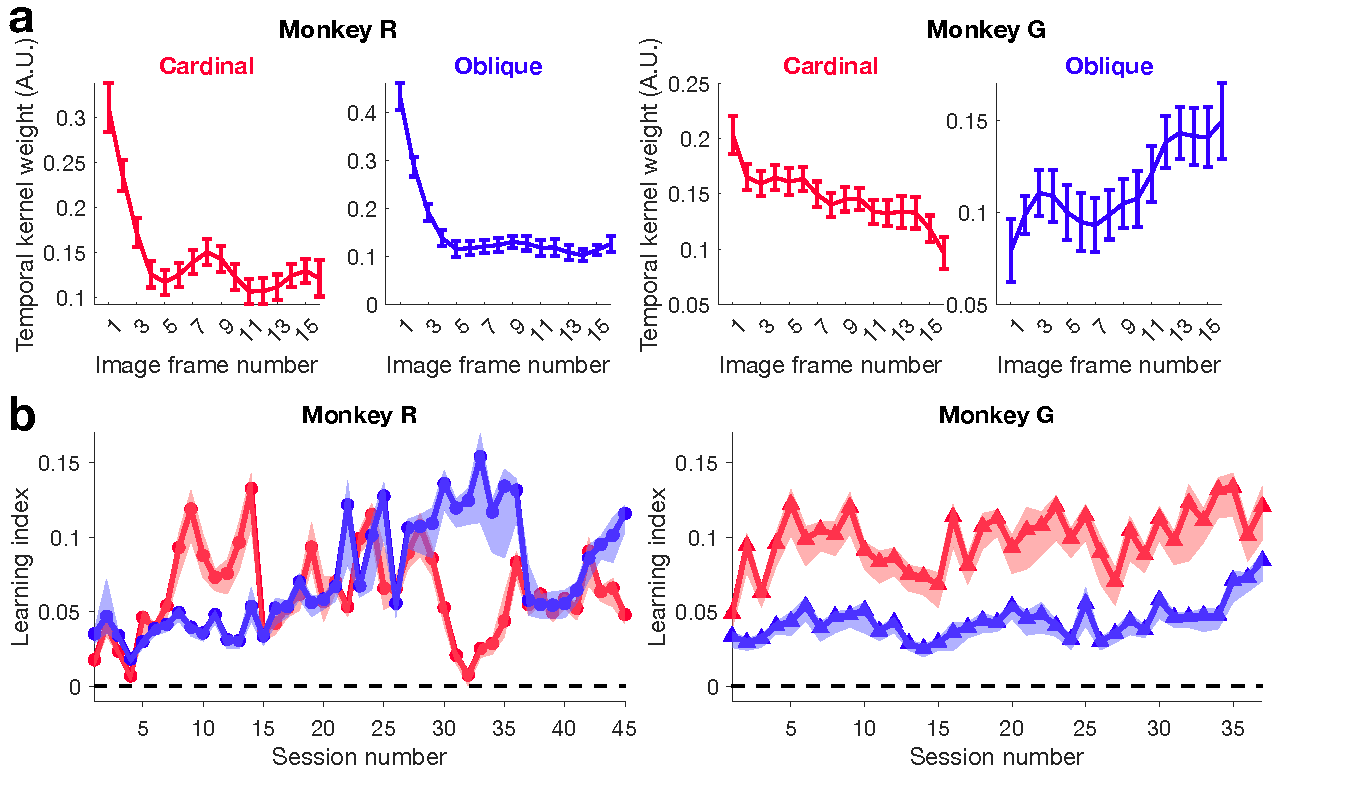
\includegraphics[width=0.8\linewidth]{figures_v2/v2_Figure_S1_suppBehav.pdf}
    \caption[Additional information on animals' behavior]{\textbf{a}: Temporal kernels of each epoch. The lines represent the average across sessions, while the error bars indicate the standard error of the mean across these sessions. \textbf{b}: Learning index for each session. Solid lines and shading represent medians and 68\% confidence intervals across 1000 bootstrap samples.}
    \label{fig:Figure_S1_additional_behav}
\end{figure}
\begin{figure}
    \centering
    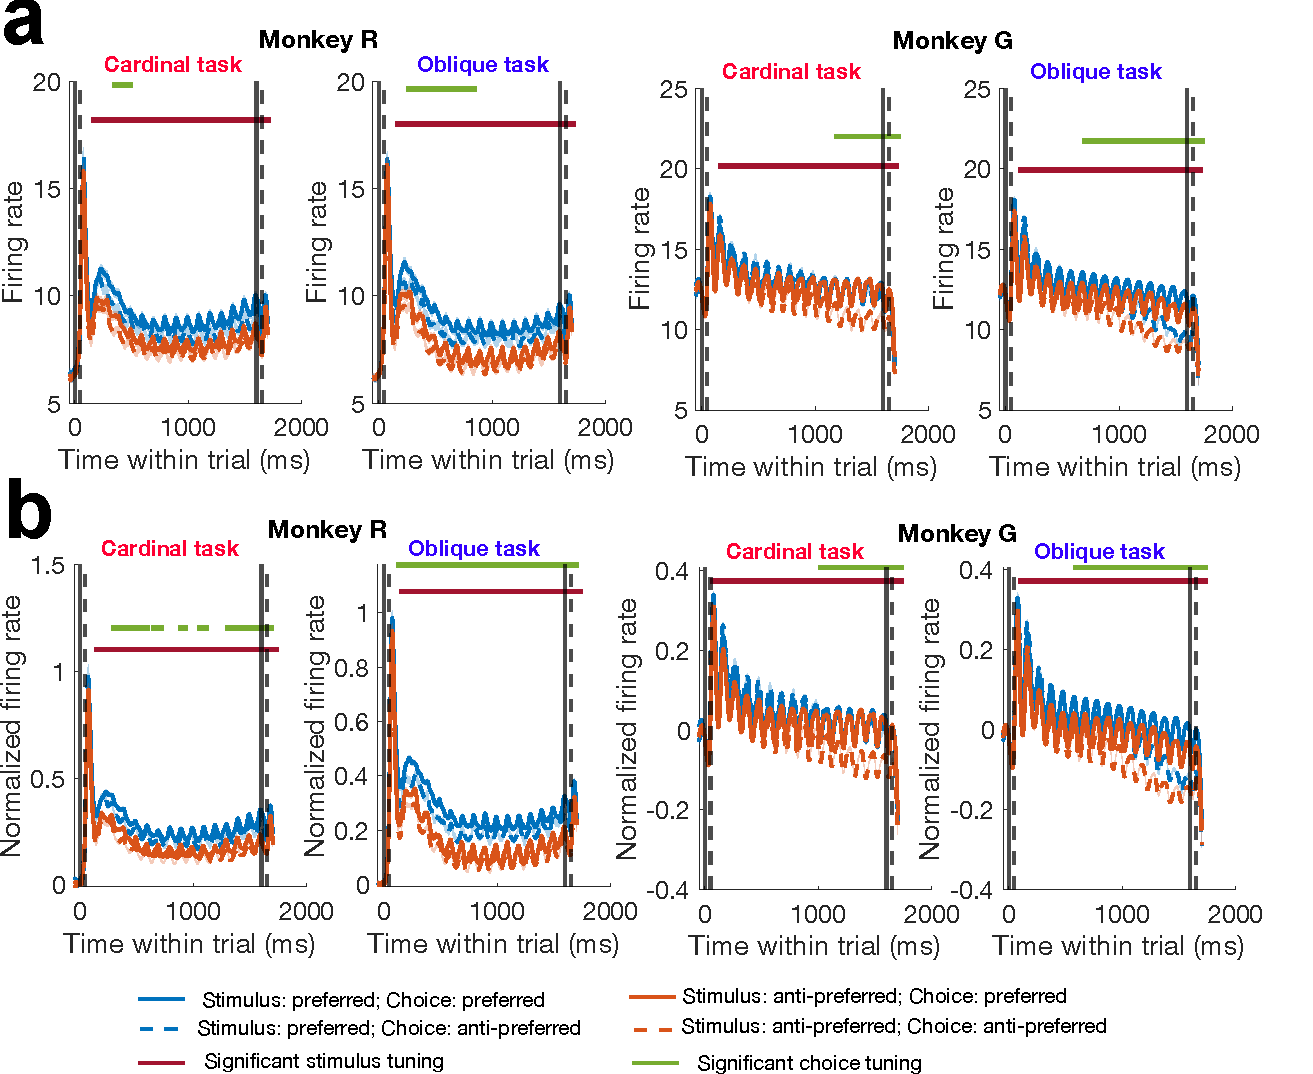
\includegraphics[width=0.8\linewidth]{figures_v2/v2_Figure_S2_PSTH.pdf}
    \caption{\textbf{Peristimulus time histogram (PSTH).} \textbf{a}: Neural response from 50 ms before stimulus onset to 100 ms after stimulus offset. Dashed vertical lines indicate stimulus onset and offset. We grouped trials into four conditions based on each unit’s preferred orientation and the chosen orientation. For each unit, the firing rates within each group were averaged to yield the mean response for each condition (represented by the blue/orange lines). The shaded areas indicate the standard error of the mean. Horizontal maroon and green bars indicate time periods when significant stimulus or choice tuning was identified with cluster-based permutation test. 
    \textbf{b}: Same as panel \textbf{a} but presenting normalized firing rate. To normalize firing rates of each unit, we computed the mean and standard deviation of firing rates during the baseline period (50 ms before stimulus onset) of all analyzed trials of a session, and used them to $z$-score firing rates of each time window (Bin size = 50 ms. A Gaussian-weighted moving average filter was applied).}
    
    \label{fig:Figure_S2_PSTH}
\end{figure}
\begin{figure}[H] %%%%% histogram of basic properties
    \centering
    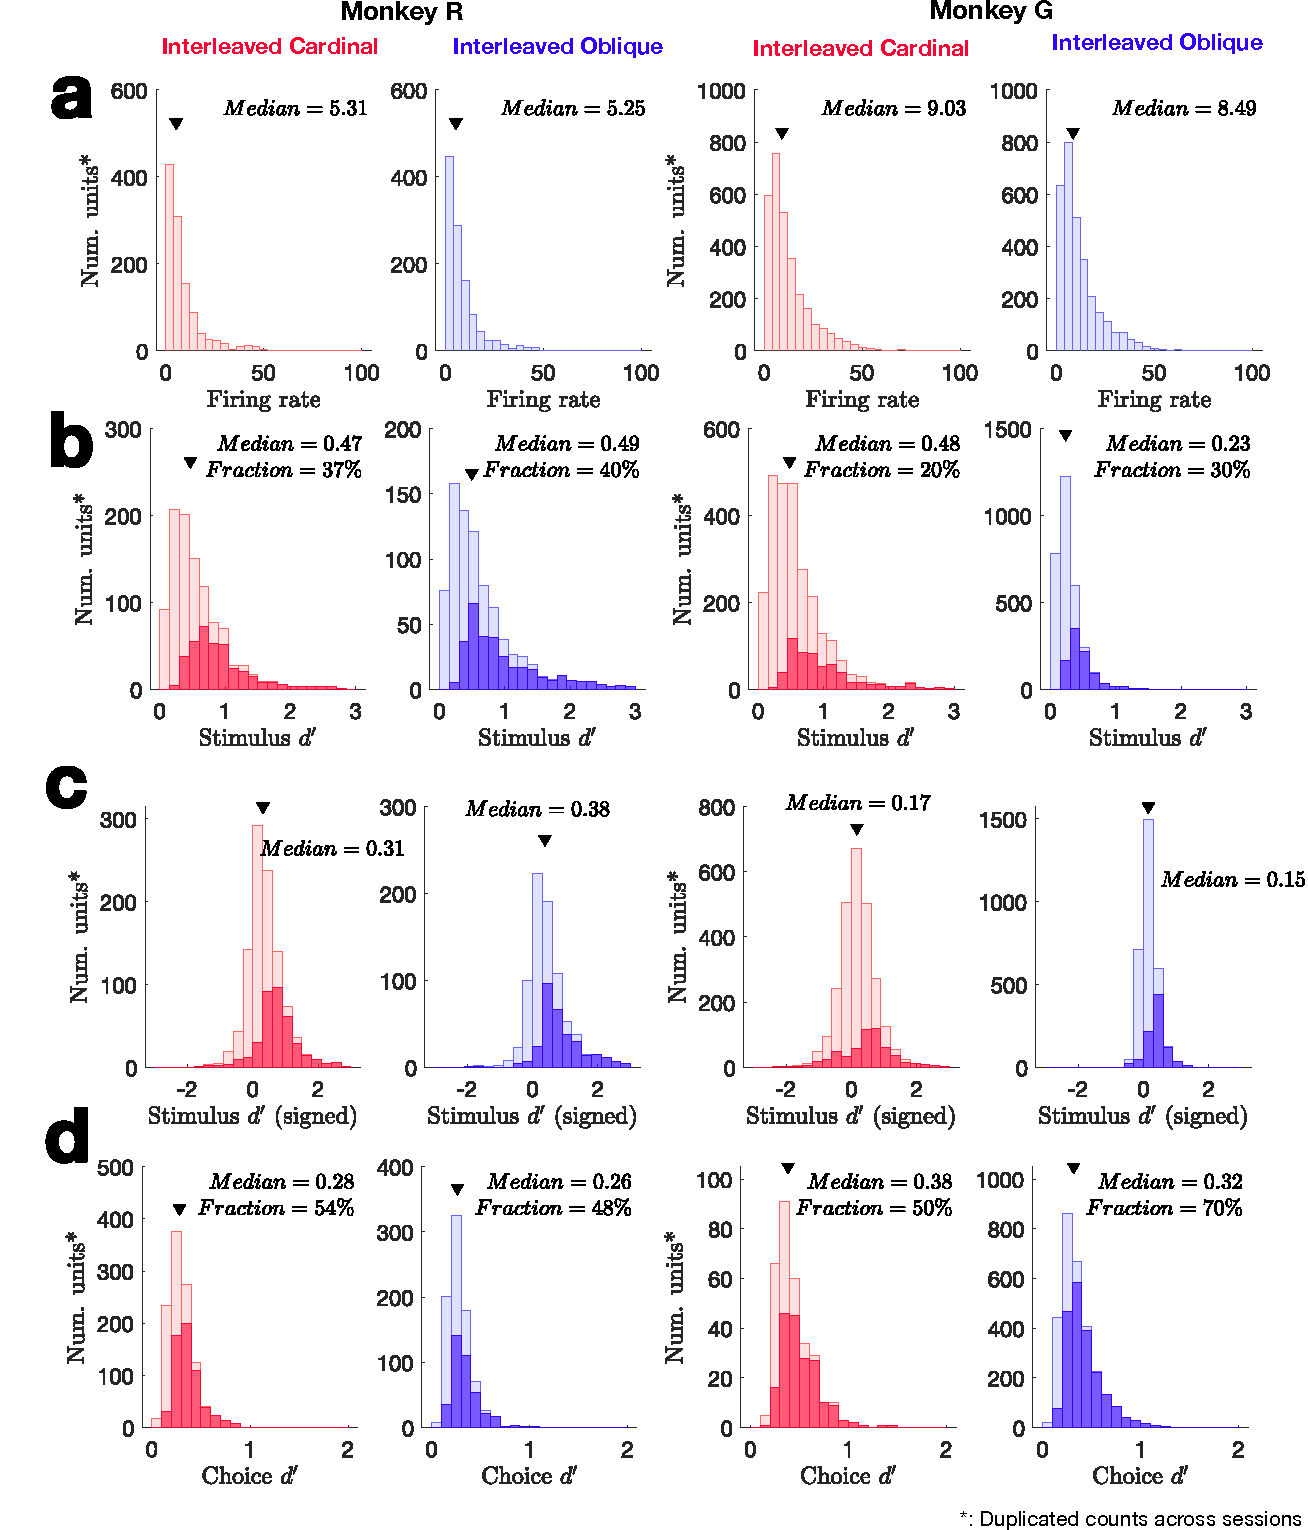
\includegraphics[width=0.8\linewidth]{figures/Figure_S1_basic_neural_histograms.pdf}
    \caption[Histograms of basic properties of analyzed units.]{\textbf{Histograms of basic properties of analyzed units.} In each panel, the triangles indicate the median values. \textbf{a}: Averaged firing rates in response to all coherence levels. \textbf{b}: Stimulus $d'$ computed with the highest coherence level for each animal (monkey R: 10\%; monkey G: 15\%). \textbf{c}: Stimulus $d'$ with sign. Positive sign indicates the unit prefer $0^\circ$ ($45^\circ$) for the cardinal (oblique) task. 
    \textbf{d}: Choice $d'$, computed for each coherence level, then averaged across coherence levels. In panels \textbf{b}, \textbf{c} and \textbf{d}, the filled histograms mark individual units with significant stimulus tuning or choice tuning (independent samples t-test).}
    \label{fig:Figure_S1_basic_neural_histograms}
\end{figure}
\begin{figure}
    \centering
    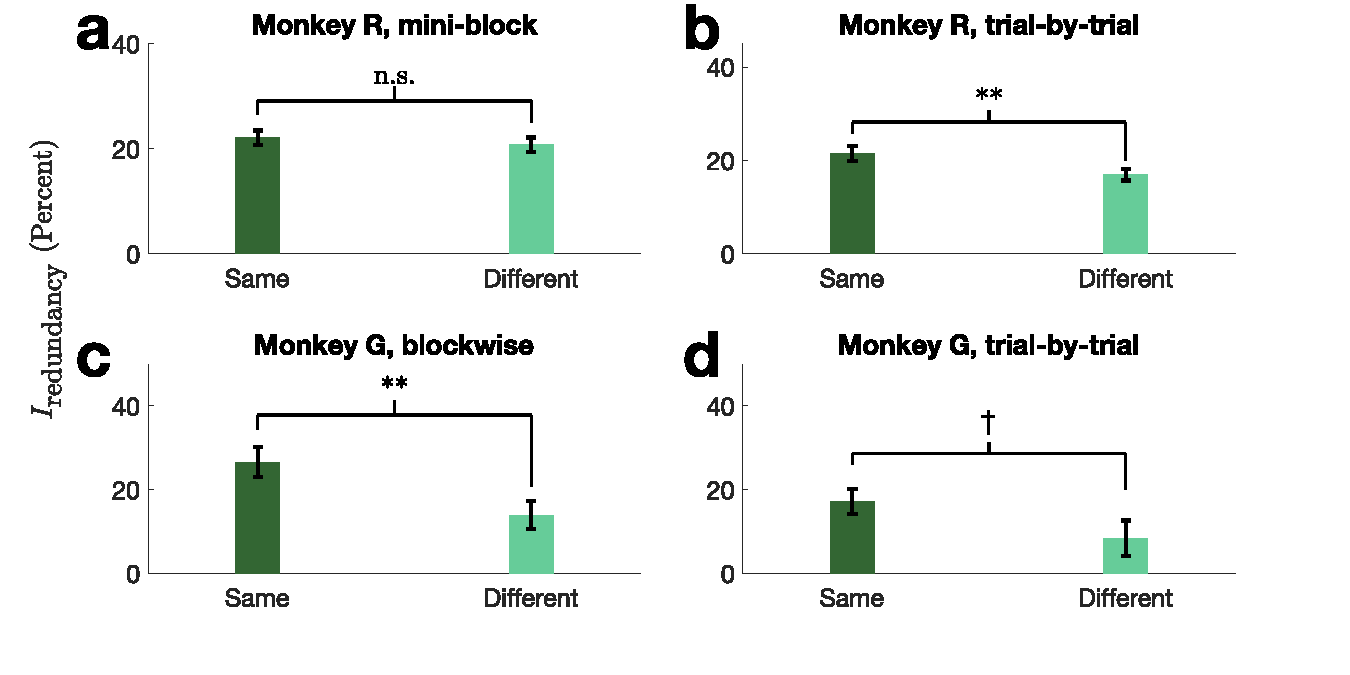
\includegraphics[width=0.8\linewidth]{figures_v2/v2_Figure_S10_informationRedundancy_percent_bytimescale.pdf}
    \caption{\textbf{Information redundancy in sessions grouped by swicthing time scale.} \textbf{a}: Monkey R sessions in which tasks switched blockwise within block size of 10-50 correct trials. \textbf{b}: Monkey R sessions in which task switched randomly, on a trial-by-trial basis. \textbf{c}: Monkey R sessions in which tasks switched blockwise within block size of 10-50 correct trials. \textbf{d}: Monkey R sessions in which task switched randomly, on a trial-by-trial basis. The task switching time scale did not significantly influence the key measurement: the difference between ``same'' and ``different'' information redundancy (independent samples t-test, monkey R: $t(36) = -1.33$, $p = \num{1.90e-01}$; monkey G: $t(35) = 0.57$, $p = \num{5.75e-01}$). Moreover, during trial-by-trial task switching sessions of monkey R, information redundancy under the same task context was still significantly higher than that under the difference task context (paired t-test, $t(22) = 2.94$, $p = \num{7.63e-03}$), and it is marginally significant for monkey G, trial-by-trial switching sessions (paired t-test, $t(11) = 1.98$, $p = \num{7.33e-02}$).}
    \label{fig:Figure_S10_redundancy_percent_bytimescale}
\end{figure}
\begin{figure}[H]
    \centering
    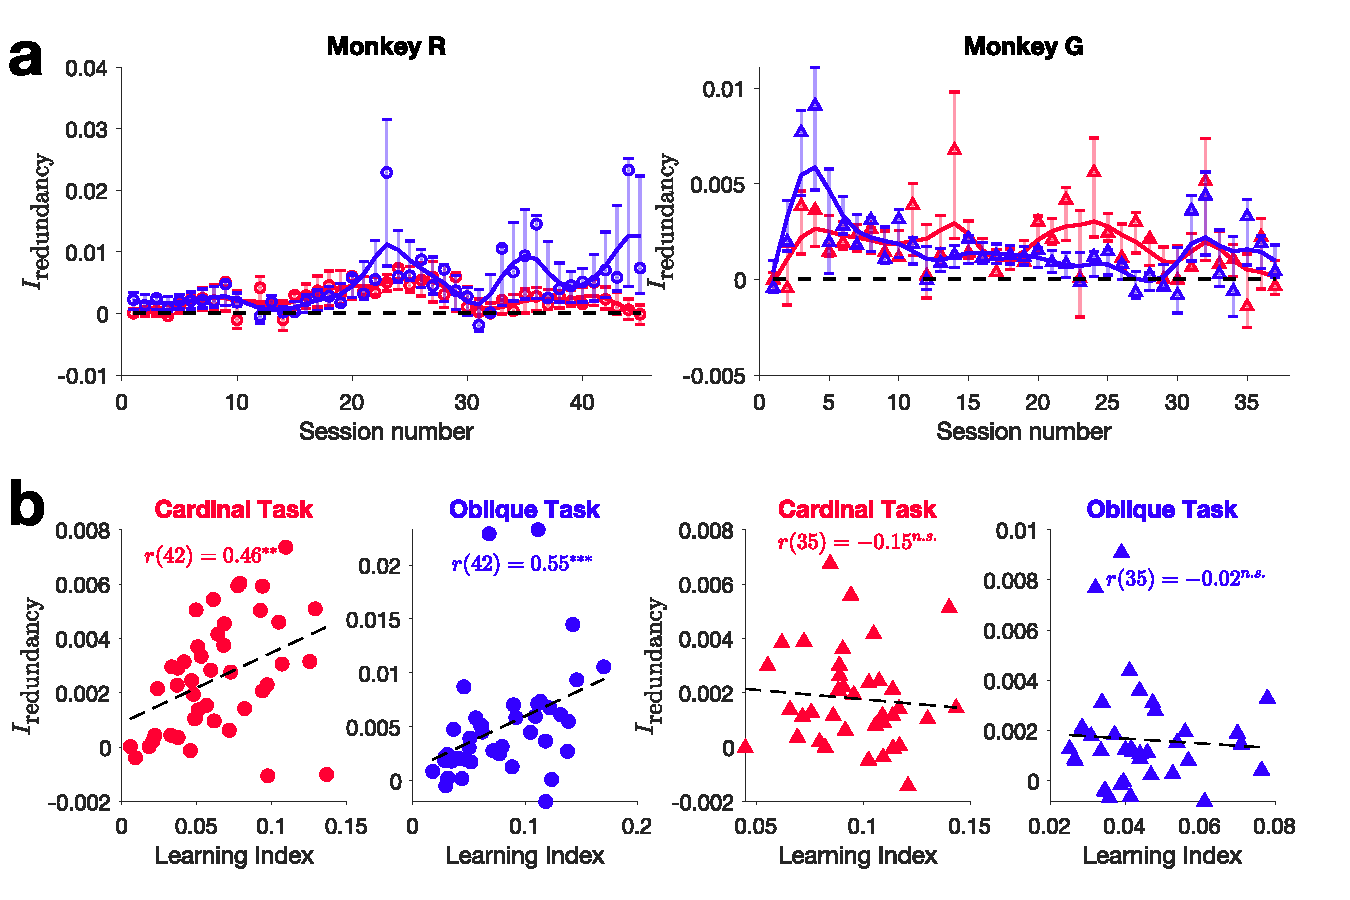
\includegraphics[width=0.8\linewidth]{figures/Figure_S6_I_redundancy_interleaved_sizeControl_interleaved.pdf}
    \caption[Information redundancy during the interleaved epoch.]{\textbf{Information redundancy during the interleaved epoch.} \textbf{a}: Time course of information redundancy over the interleaved epoch. The error bars indicate 68\% confidence intervals across Bootstrap samples of units. \textbf{b}: Scatter plot between information redundancy and learning index. Each dot represents a session. Black dashed lines are linear regression fits across sessions. Correlation coefficients are from Spearman's rank correlation.(Significance levels: \protect{$^{*}p < 0.05$, $^{**}p < 0.01$, $^{***}p < 0.001$})}
 \label{fig:Figure_S6_I_redundancy_interleaved_sizeControl_interleaved}
\end{figure}

\begin{figure}
    \centering
    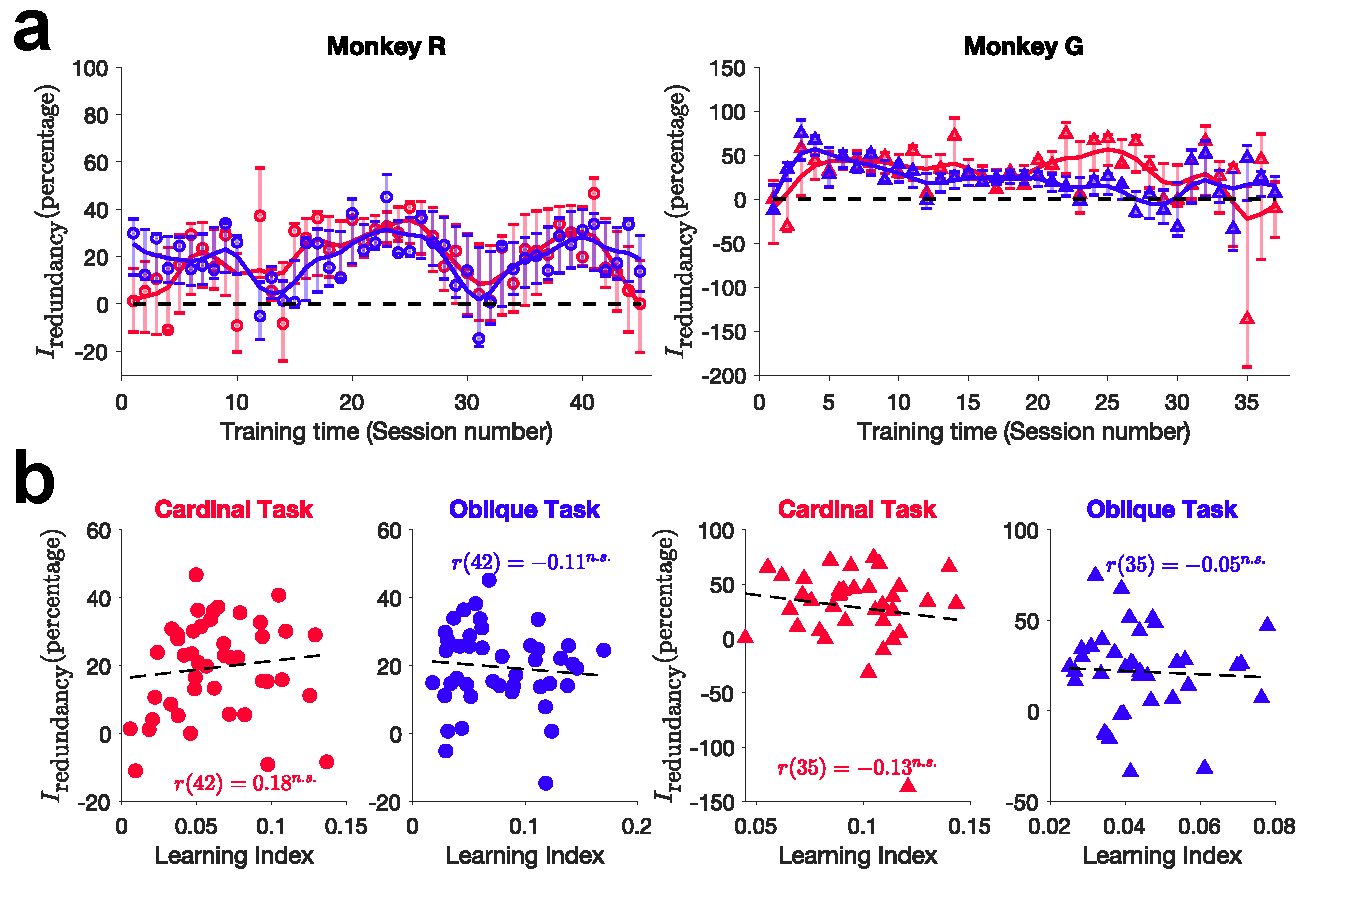
\includegraphics[width=0.8\linewidth]{figures/Figure_S5_I_redundancy_percentage_interleaved_sizeControl_interleaved.pdf}
    \caption[Information redundancy as percentage of shuffled Fisher information.]{\textbf{Information redundancy as percentage of shuffled Fisher information.}Same as figure~\ref{fig:Figure_S6_I_redundancy_interleaved_sizeControl_interleaved}, but information redundancy was normalized to be the percentage of $\Is$.}
    \label{fig:Figure_S5_I_redundancy_percentage_interleaved_sizeControl_interleaved}
\end{figure}

\begin{figure}[H]
    \centering
    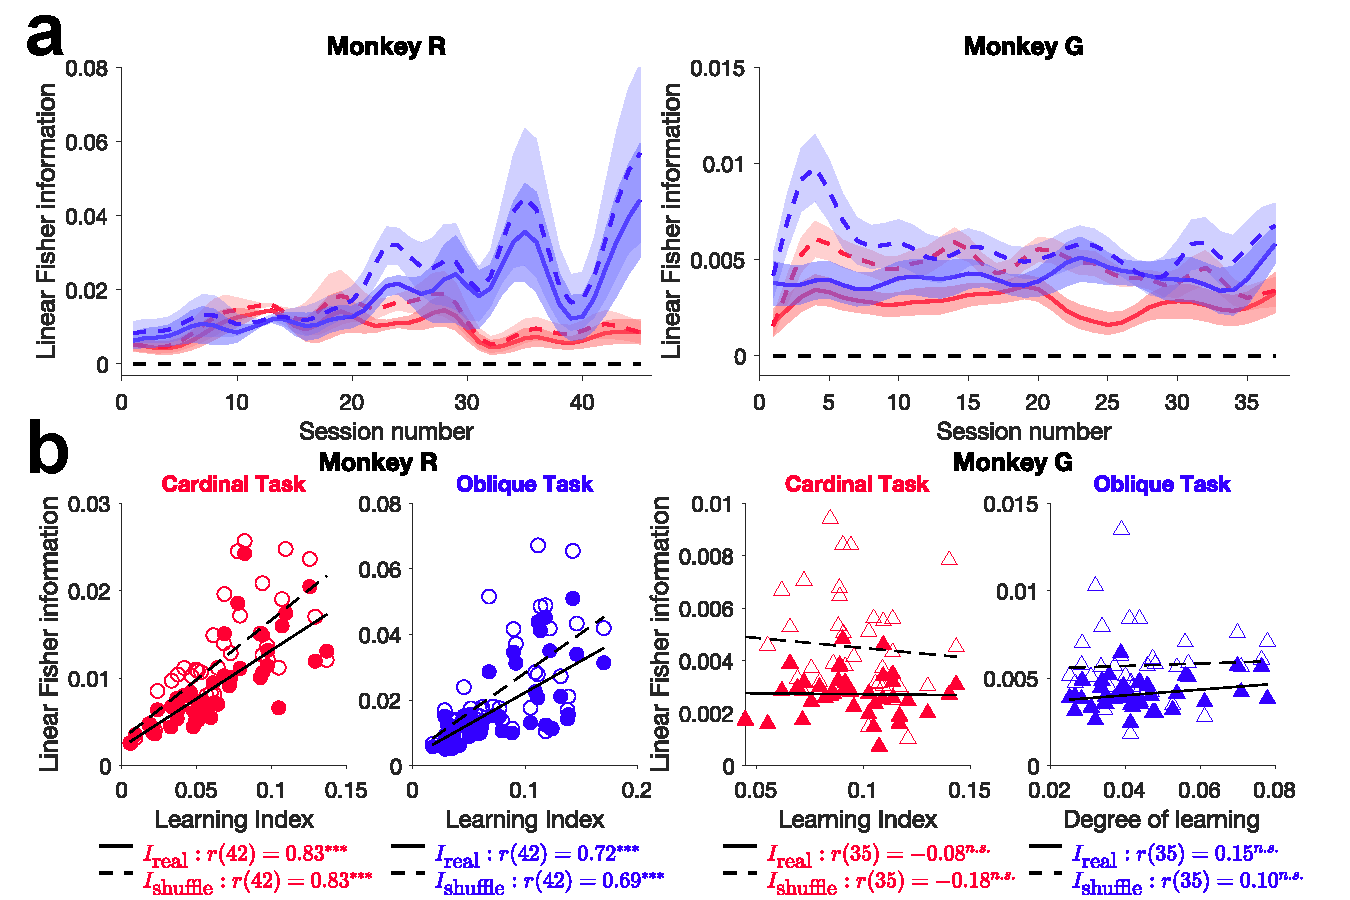
\includegraphics[width=0.8\linewidth]{figures/Figure_S7_FisherInfo_sizeControl_nobehav.pdf}
    \caption[The real and shuffled linear Fisher information during the interleaved epoch.]{\textbf{The real and shuffled linear Fisher information during the interleaved epoch.} \textbf{a} Time course of $\Ir$ and $\Is$ over the interleaved epoch. Shaded areas: 68\% across Bootstrap samples. 
    \textbf{b}: Correlation between learning index $\Ir$ and $\Is$, respectively. One dot per session. Black lines are a linear regression fit across sessions, solid for $\Ir$ and dashed for $\Is$. (Significance levels: $^{*}p < 0.05$, $^{**}p < 0.01$, $^{***}p < 0.001$)}
    \label{fig:Figure_S7_FisherInfo_sizeControl_nobehav}
\end{figure}

\begin{figure}[H]
    \centering
    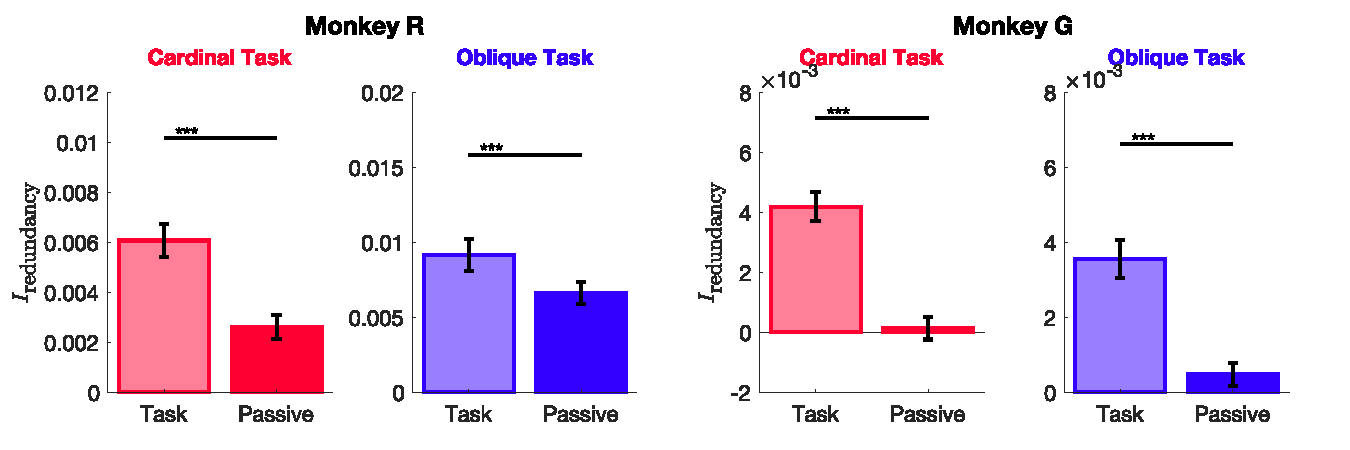
\includegraphics[width=0.8\linewidth]{figures/Figure_S9_passive_task_Iredundancy_sizeControl.pdf}
    \caption[Compare $\Idelta$ during task-performing and passive-viewing in the interleaved epoch.]{\textbf{Compare $\Idelta$ during task-performing and passive-viewing in the interleaved epoch.} The bar plots averaged \protect{$\Idelta$} across sessions in each learning stage when the animals were performing the task or passively viewing the stimulus. Error bars indicate the standard error of the mean across sessions. Note that task-performing data were separated into 400 ms time bins and then averaged to match the stimulus duration in passive viewing data. (Significance levels: \protect{$^{*}p < 0.05$, $^{**}p < 0.01$, $^{***}p < 0.001$})} \label{fig:Figure_S9_passive_task_Iredundancy_sizeControl}
\end{figure}

\begin{figure}[H]
    \centering
    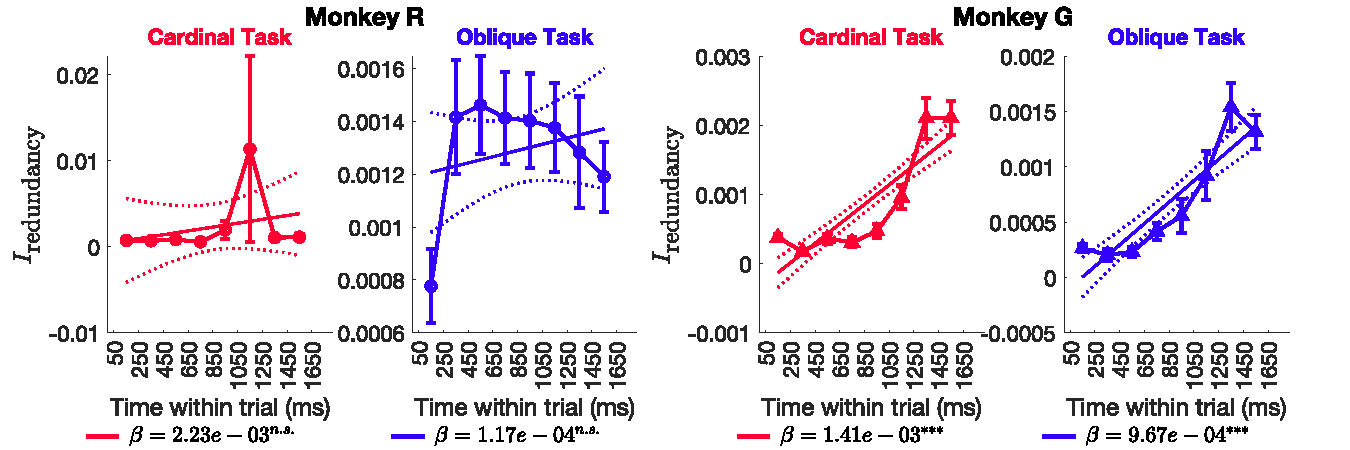
\includegraphics[width=0.8\linewidth]{figures/Figure_S8_withinTrial_Iredundancy_sizeControl.pdf}
    \caption[Within-trial dynamic of information redundancy during the interleaved epoch.]{\textbf{Within-trial dynamic of information redundancy during the interleaved epoch.} $\Idelta$ for each 200~ms time bin within a trial in the interleaved epoch, controlled for population size. $\beta$ is the regression coefficient: $\Idelta$ vs time bin. Error bars indicate the standard error of the mean. across sessions (Significance levels: $^{*}p < 0.05$, $^{**}p < 0.01$, $^{***}p < 0.001$)}
    \label{fig:Figure_S8_withinTrial_Iredundancy_sizeControl}
\end{figure}


\begin{figure}[H]
    \centering
    
\includegraphics[width=0.8\linewidth]{figures/Figure_S2_empirical_barplot_perCohr.pdf}
    \caption[Linear Fisher information under task switching in the empirical data measured per coherence level.]{ \textbf{Linear Fisher information under task switching in the empirical data measured per coherence level.}Same as Fig.~\ref{fig:Figure_3_empirical_barplot}, but each data sample represents the result based on one coherence level.}
    \label{fig:Figure_S2_empirical_barplot_perCohr}
\end{figure}


\begin{figure}[H]
    \centering
    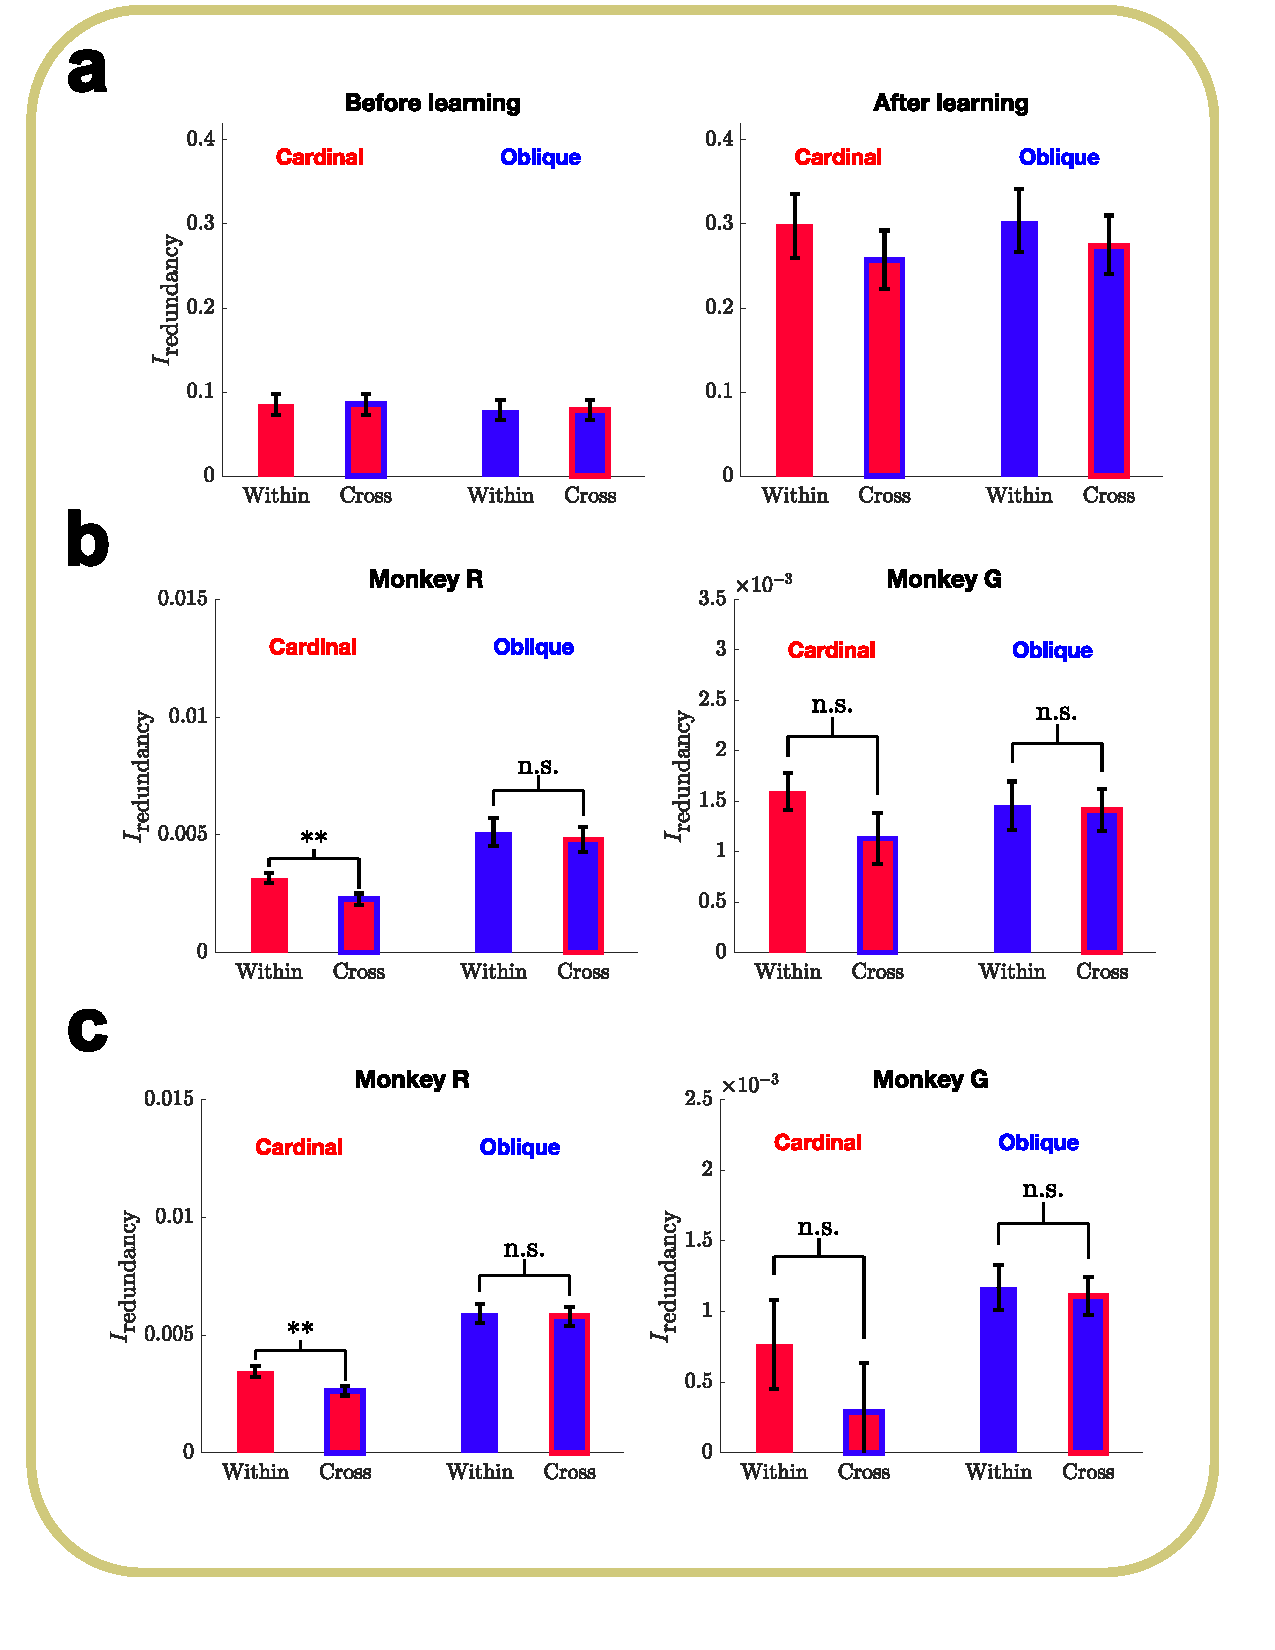
\includegraphics[width=0.8\linewidth]{figures/Figure_S3_I_redundacy_raw.pdf}
    \caption[Raw information redundancy without normalization.]{\textbf{Raw information redundancy without normalization.} \textbf{a}: $\Idelta$ in the generative Bayesian inference model. \textbf{b}: $\Idelta$ in the empirical data. One data point represents one session with results from multiple coherence levels combined (Paired t-test, within v.s. cross: monkey R cardinal, $t(37) = 2.84$, $p = \num{7.25e-03}$; monkey R oblique: $t(37) = 0.77$, $p = \num{4.48e-01}$; monkey G cardinal: $t(36) = 2.02$, $p = \num{5.05e-02}$; monkey G oblique: $t(36) = 0.19$, $p = \num{8.51e-01}$)
    \textbf{c}:  $\Idelta$ in the empirical data. One data point represents one coherence level.(Paired t-test, within vs. cross:  monkey R cardinal, $t(114) = 3.11$, $p = \num{2.35e-03}$; monkey R oblique:  $t(114) = 0.38$, $p = \num{7.08e-01}$; monkey G cardinal:  $t(127) = 1.87$, $p = \num{6.37e-02}$; monkey G oblique:  $t(106) = 0.33$, $p = \num{7.43e-01}$)
}
    \label{fig:Figure_S3_I_redundacy_raw}
\end{figure}


% An appendix contains supplementary information that is not an essential part of the text itself but which may be helpful in providing a more comprehensive understanding of the research problem or it is information that is too cumbersome to be included in the body of the paper.

%%=============================================%%
%% For submissions to Nature Portfolio Journals %%
%% please use the heading ``Extended Data''.   %%
%%=============================================%%

%%=============================================================%%
%% Sample for another appendix section			       %%
%%=============================================================%%

%% \section{Example of another appendix section}\label{secA2}%
%% Appendices may be used for helpful, supporting or essential material that would otherwise 
%% clutter, break up or be distracting to the text. Appendices can consist of sections, figures, 
%% tables and equations etc.

\end{appendices}

%%===========================================================================================%%
%% If you are submitting to one of the Nature Portfolio journals, using the eJP submission   %%
%% system, please include the references within the manuscript file itself. You may do this  %%
%% by copying the reference list from your .bbl file, paste it into the main manuscript .tex %%
%% file, and delete the associated \verb+\bibliography+ commands.                            %%
%%===========================================================================================%%

\bibliography{references}% common bib file
%% if required, the content of .bbl file can be included here once bbl is generated
%%\input sn-article.bbl

\end{document}
